\section{相关理论基础\label{相关工作}}

\subsection{目标检测的理论基础与算法}

\subsubsection{双阶段目标检测算法}

双阶段目标检测算法采用分步处理的策略,可分为区域候选生成阶段和区域分类识别阶段。在第一阶段,算法主要负责生成一系列可能包含目标物体的候选区域。这些候选区域是基于图像的局部特征和先验知识来提取的,例如在一些传统算法中利用滑动窗口结合图像金字塔的方式,或者在基于深度学习的算法中采用特定的区域生成网络(RPN,Region Proposal Network)来快速产生大量的候选区域。区域生成网络会扫描输入图像,基于图像的边缘、纹理等特征来预测可能的目标位置,生成大小不一、位置各异的候选区域提议(proposals)。这些候选区域通常具有一定的,数量例如几千个不等,它们覆盖了图像中可能存在的各种目标物体的潜在位置和尺度。

在第二阶段,将第一阶段生成的候选区域作为输入,对其进行更深入的特征提取和分类识别。此时,算法会针对每个候选区域提取更具有判别力的特征,通常是利用深度卷积神经网络对候选区域内的图像内容进行特征编码。然后,利用这些特征来判断该区域是否属于某一目标类别,并进一步对目标的位置进行精确回归调整,优化候选区域的边界框坐标,使其更准确地框定目标物体。这一阶段的处理通常涉及复杂的网络结构和大量的计算,目的是在候选区域的基础上实现高精度的目标分类和定位。

随着深度学习技术在计算机视觉领域的广泛应用,基于深度学习的特征提取方法成为双阶段目标检测算法的核心部分。深度卷积神经网络(CNN)\cite{cnn}通过多层卷积和池化操作,能够自动学习到图像的层次化特征表示。在双阶段目标检测算法中,通常采用预训练的深度 CNN 作为特征提取器,例如 VGGNet\cite{simonyan2014very}、ResNet \cite{he2016deep}等知名网络架构。这些网络经过在大规模图像数据集上的预训练,已经学习到了图像的通用特征表示,包括边缘、纹理、形状等低层特征以及更抽象的语义特征。

在区域候选生成阶段,特征提取网络会对输入图像进行初步的特征编码,为后续的候选区域生成提供特征基础。而在区域分类识别阶段,会进一步利用更深的网络结构对候选区域内的特征进行提取和压缩,以便更准确地区分不同目标类别。深度学习的特征提取方法相较于传统的手工特征(如 HOG、SIFT 等)\cite{Haar_like}具有明显的优势,能够更好地适应不同场景下目标物体的复杂变化,捕捉到更丰富的目标特征信息,从而为后续的目标分类和定位提供更有力的支持。

R-CNN \cite{girshick2014rich, fast_rcnn,faster_rcnn, mask_rcnn}是双阶段目标检测算法的开创性工作。R-CNN 网络结构如图 \ref{fig:rcnn} 所示。它首先利用选择性搜索算法在输入图像中生成约 2000 个候选区域。选择性搜索算法基于图像的分割和合并策略,根据颜色、纹理、大小等相似性将图像分割为多个区域,然后逐步合并相似区域,从而生成一系列不同尺度和形状的候选区域。接着,对每个候选区域进行归一化处理,调整其大小使其适应预定义的深度 CNN 输入尺寸。将归一化后的候选区域输入到深度 CNN 中(如 AlexNet)进行特征提取,得到每个候选区域的特征向量。最后,利用支持向量机(SVM)\cite{svm}分类器对候选区域进行分类,判断其属于哪个目标类别,并通过线性回归模型对候选区域的边界框坐标进行微调,以提高目标定位的精度。

\begin{figure}[htbp]
    \centering
    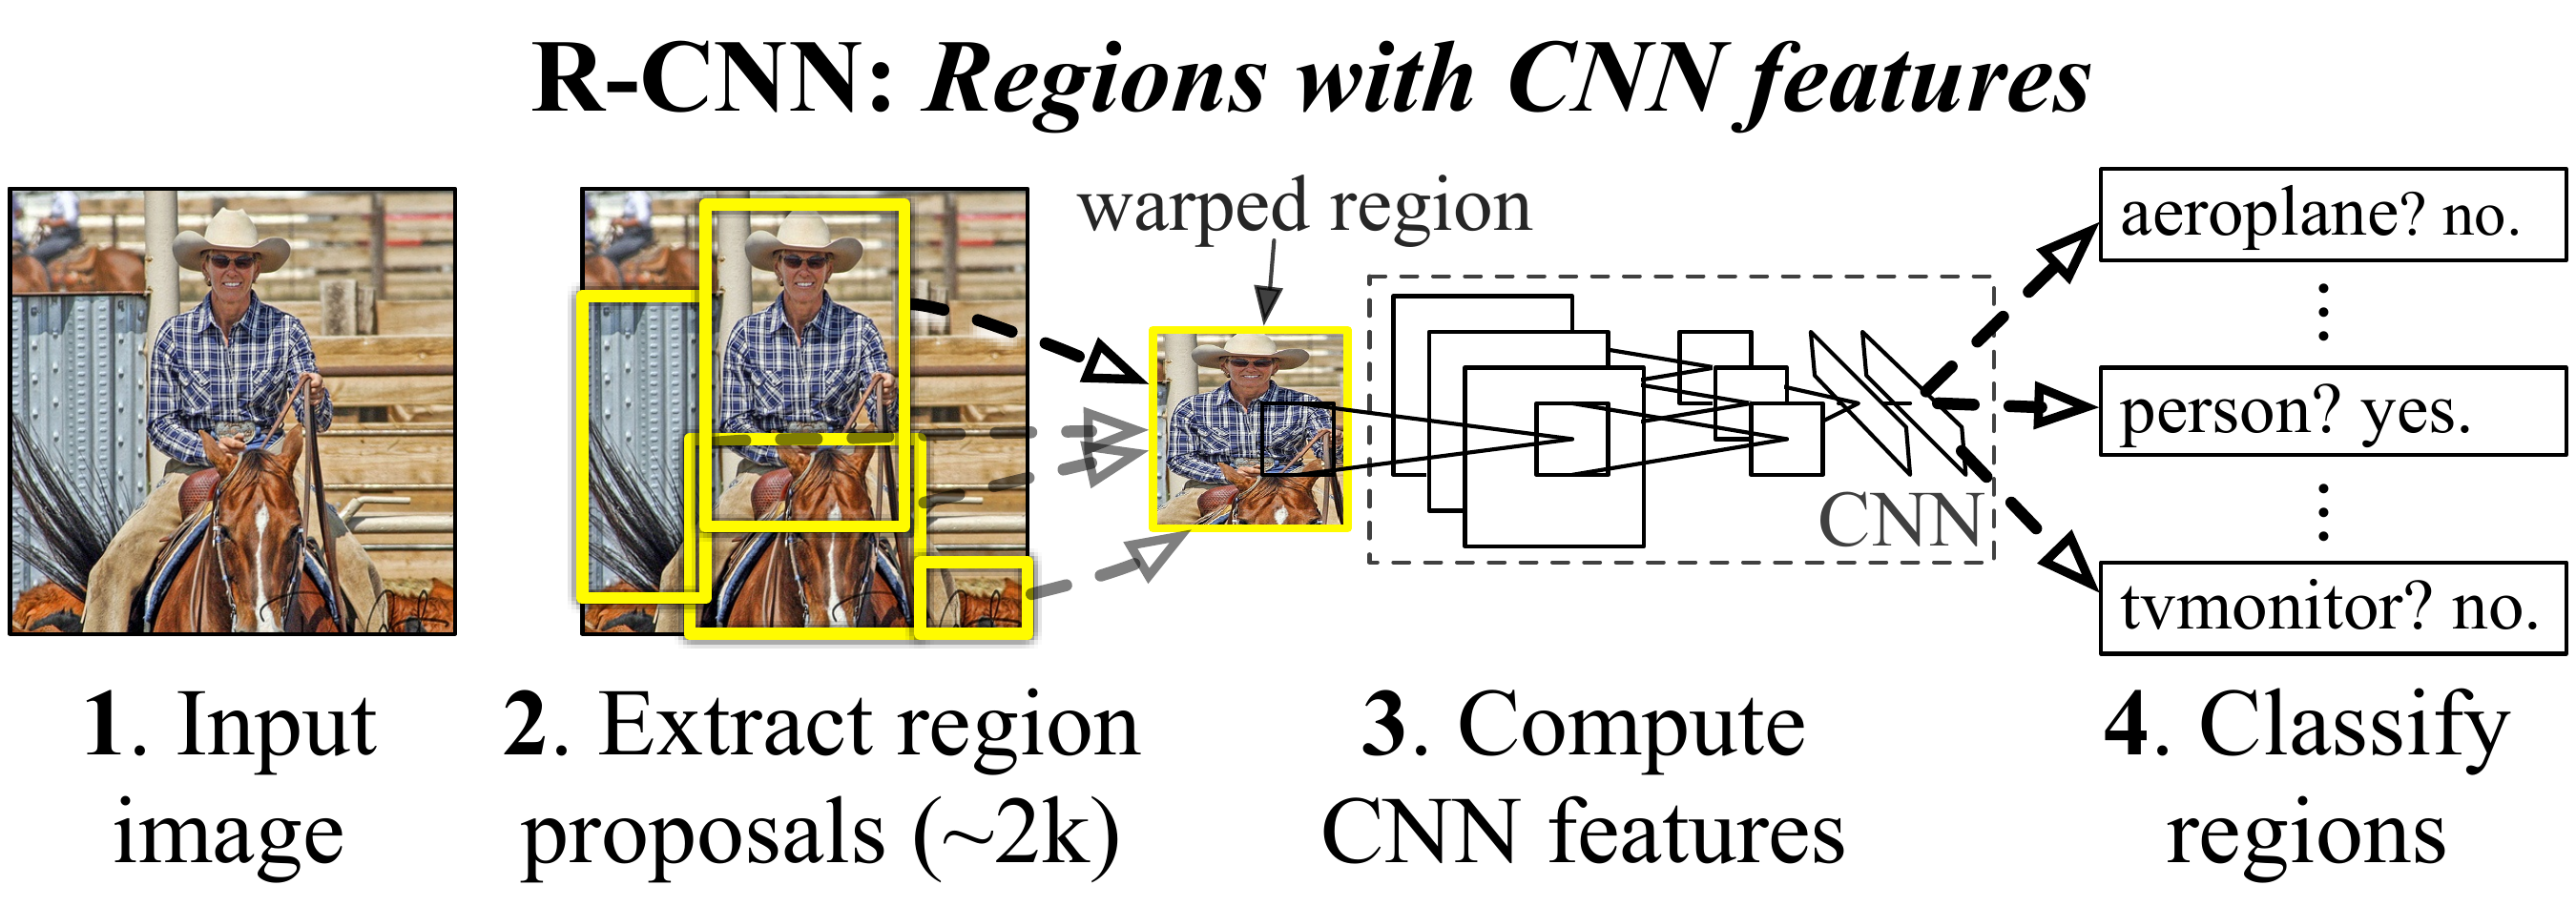
\includegraphics[width=0.7\textwidth]{../figure/rcnn.png}
    \captionsetup{font=footnotesize}
    \bicaption{RCNN 网络\cite{girshick2014rich}}{RCNN Net}
    \label{fig:rcnn}
\end{figure}

R-CNN 的提出在目标检测领域取得了重大突破,相较于传统的基于手工特征的目标检测方法,它在 PASCAL VOC 等基准数据集上取得了显著的性能提升。然而,R-CNN 也存在一些明显的不足。例如,候选区域生成过程较为耗时,选择性搜索算法的效率较低;对每个候选区域单独进行 CNN 特征提取导致计算冗余,因为大量候选区域之间存在重叠区域,重复计算了相同的图像特征,使得整个算法的处理速度较慢,难以满足实时应用的需求。

为了解决 R-CNN 中计算效率低下的问题,Fast R-CNN 对算法流程进行了改进。Fast R-CNN 网络结构如图 \ref{fig:fastrcnn} 所示。它不再对每个候选区域单独进行 CNN 特征提取,而是先将整个图像输入到深度 CNN 中进行特征提取,得到一个卷积特征图。然后,在这个卷积特征图上利用区域候选生成方法(如选择性搜索)生成候选区域,并将每个候选区域映射到卷积特征图上对应的区域。通过在卷积特征图上对候选区域进行感兴趣区域池化(ROIPooling)操作,将不同大小的候选区域池化到相同尺寸的特征向量。最后,将这些固定尺寸的特征向量输入到全连接层,进行目标分类和边界框回归。

\begin{figure}[htbp]
    \centering
    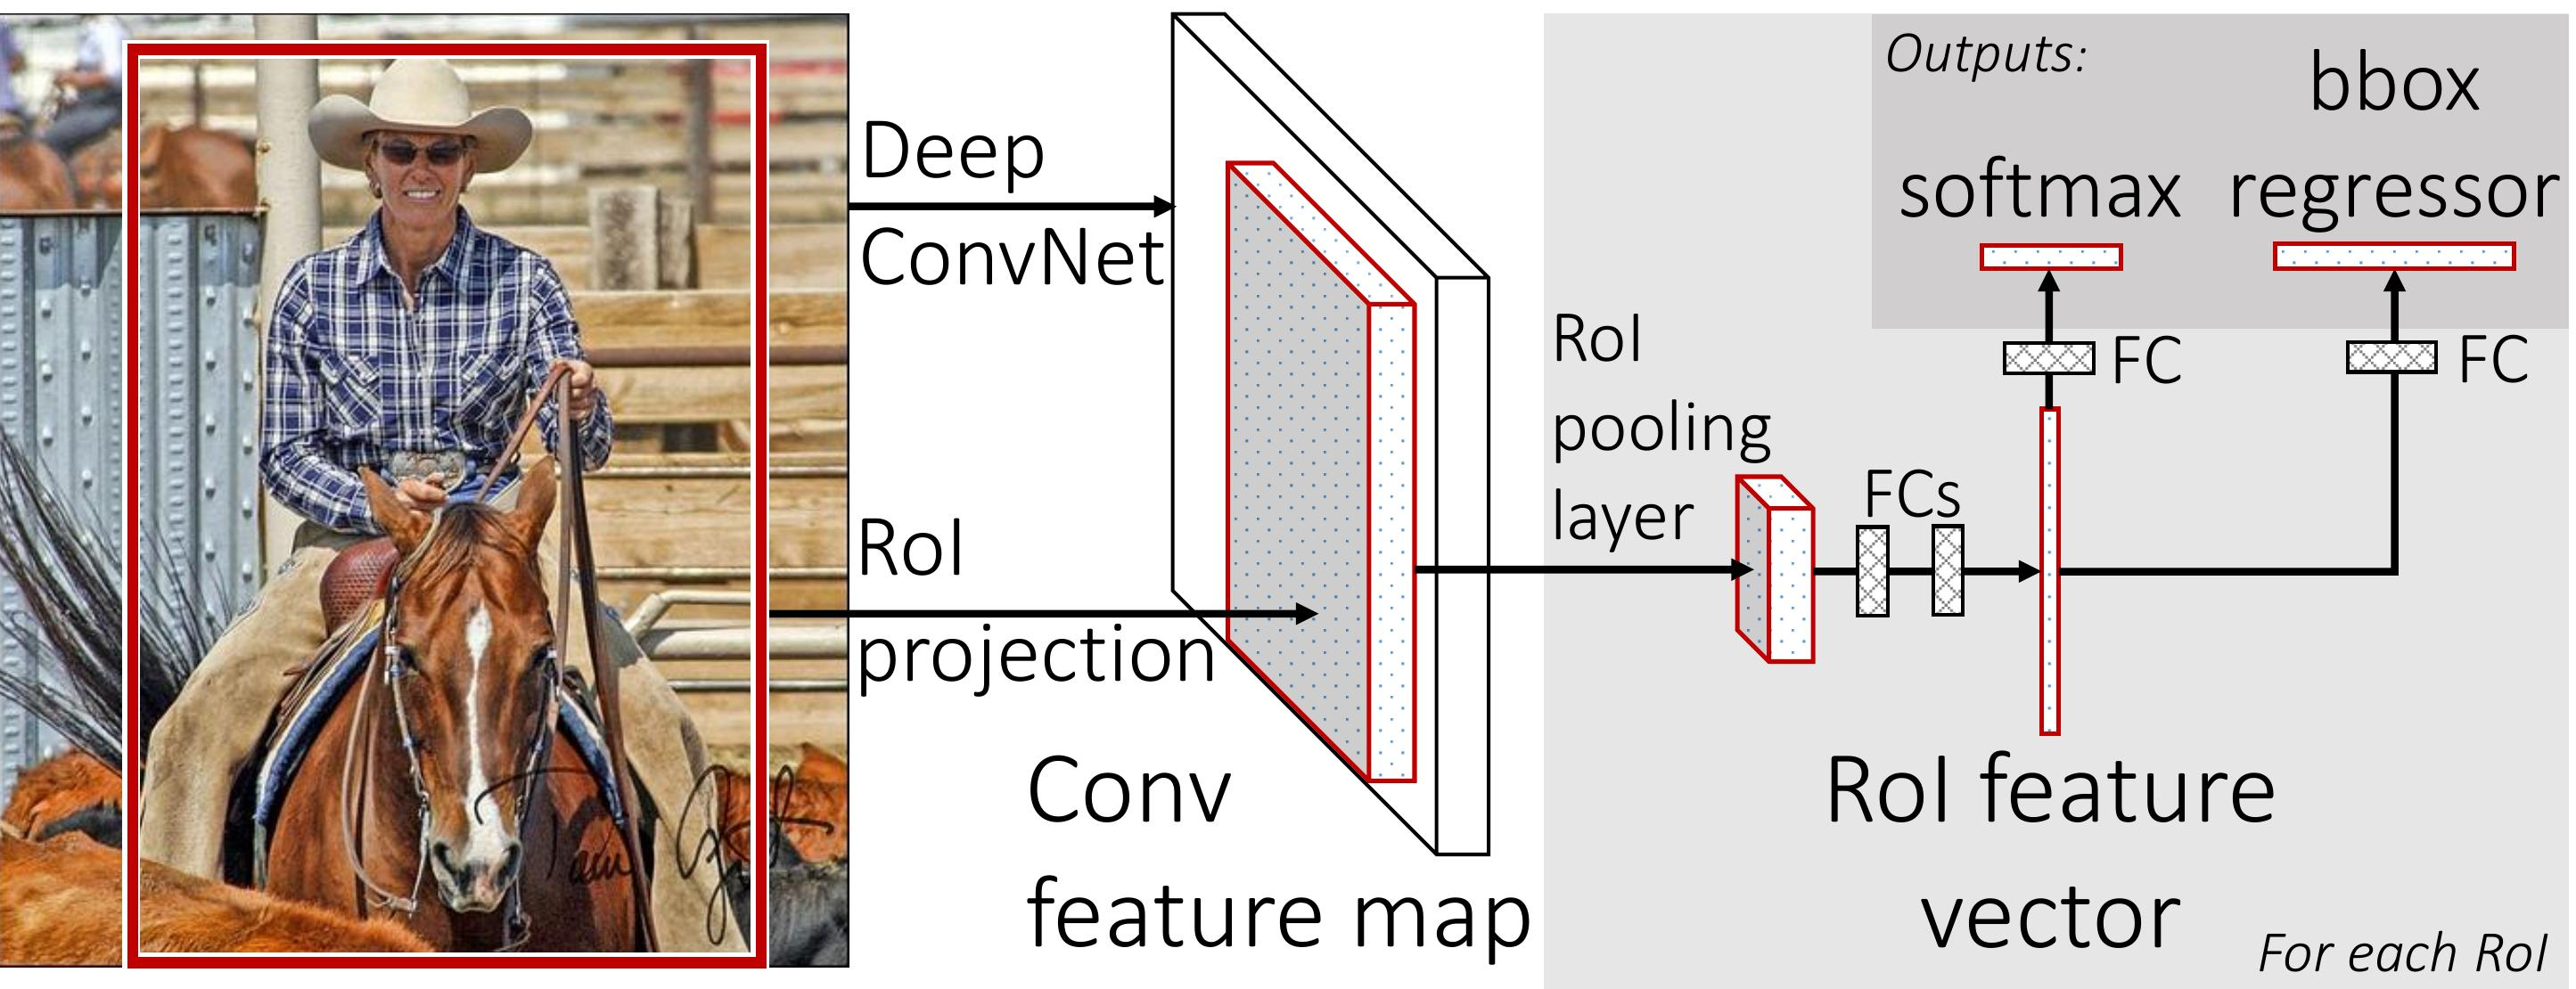
\includegraphics[width=0.7\textwidth]{../figure/fastrcnn.png}
    \captionsetup{font=footnotesize}
    \bicaption{Fast RCNN 网络\cite{fast_rcnn}}{Some descriptions of the pictures in question.}
    \label{fig:fastrcnn}
\end{figure}

这种改进方式大大提高了算法的处理速度,因为它避免了对每个候选区域重复进行卷积操作,而是在整个图像特征提取的基础上进行后续处理,有效地减少了计算量。同时,Fast R-CNN 还在训练过程中采用了多任务损失函数,将目标分类和边界框回归同时进行联合训练,进一步提升了模型的性能。然而,尽管 Fast R-CNN 在效率方面有了显著提升,但候选区域生成阶段仍然依赖选择性搜索算法,这在一定程度上限制了算法的速度和实时性。

Faster R-CNN 是在 Fast R-CNN 的基础上进一步引入了区域候选网络(RPN),实现了候选区域的自动生成,从而彻底摒弃了传统的目标区域候选生成方法。 Faster R-CNN 网络结构如图 \ref{fig:fasterrcnn} 所示。RPN 是一个全卷积网络,直接以卷积特征图为输入,通过在特征图上滑动窗口的方式,在每个位置同时预测候选区域的位置坐标和该区域属于目标物体前景或背景的概率分数。RPN 生成的候选区域经过非极大值抑制(NMS)处理后,筛选出最有可能包含目标的候选区域,并将这些区域通过 ROIPooling 层映射到固定尺寸的特征图,然后依次输入到全连接层进行目标分类和边界框回归,与 Fast R-CNN 的后续处理流程类似。

\begin{figure}[htbp]
    \centering
    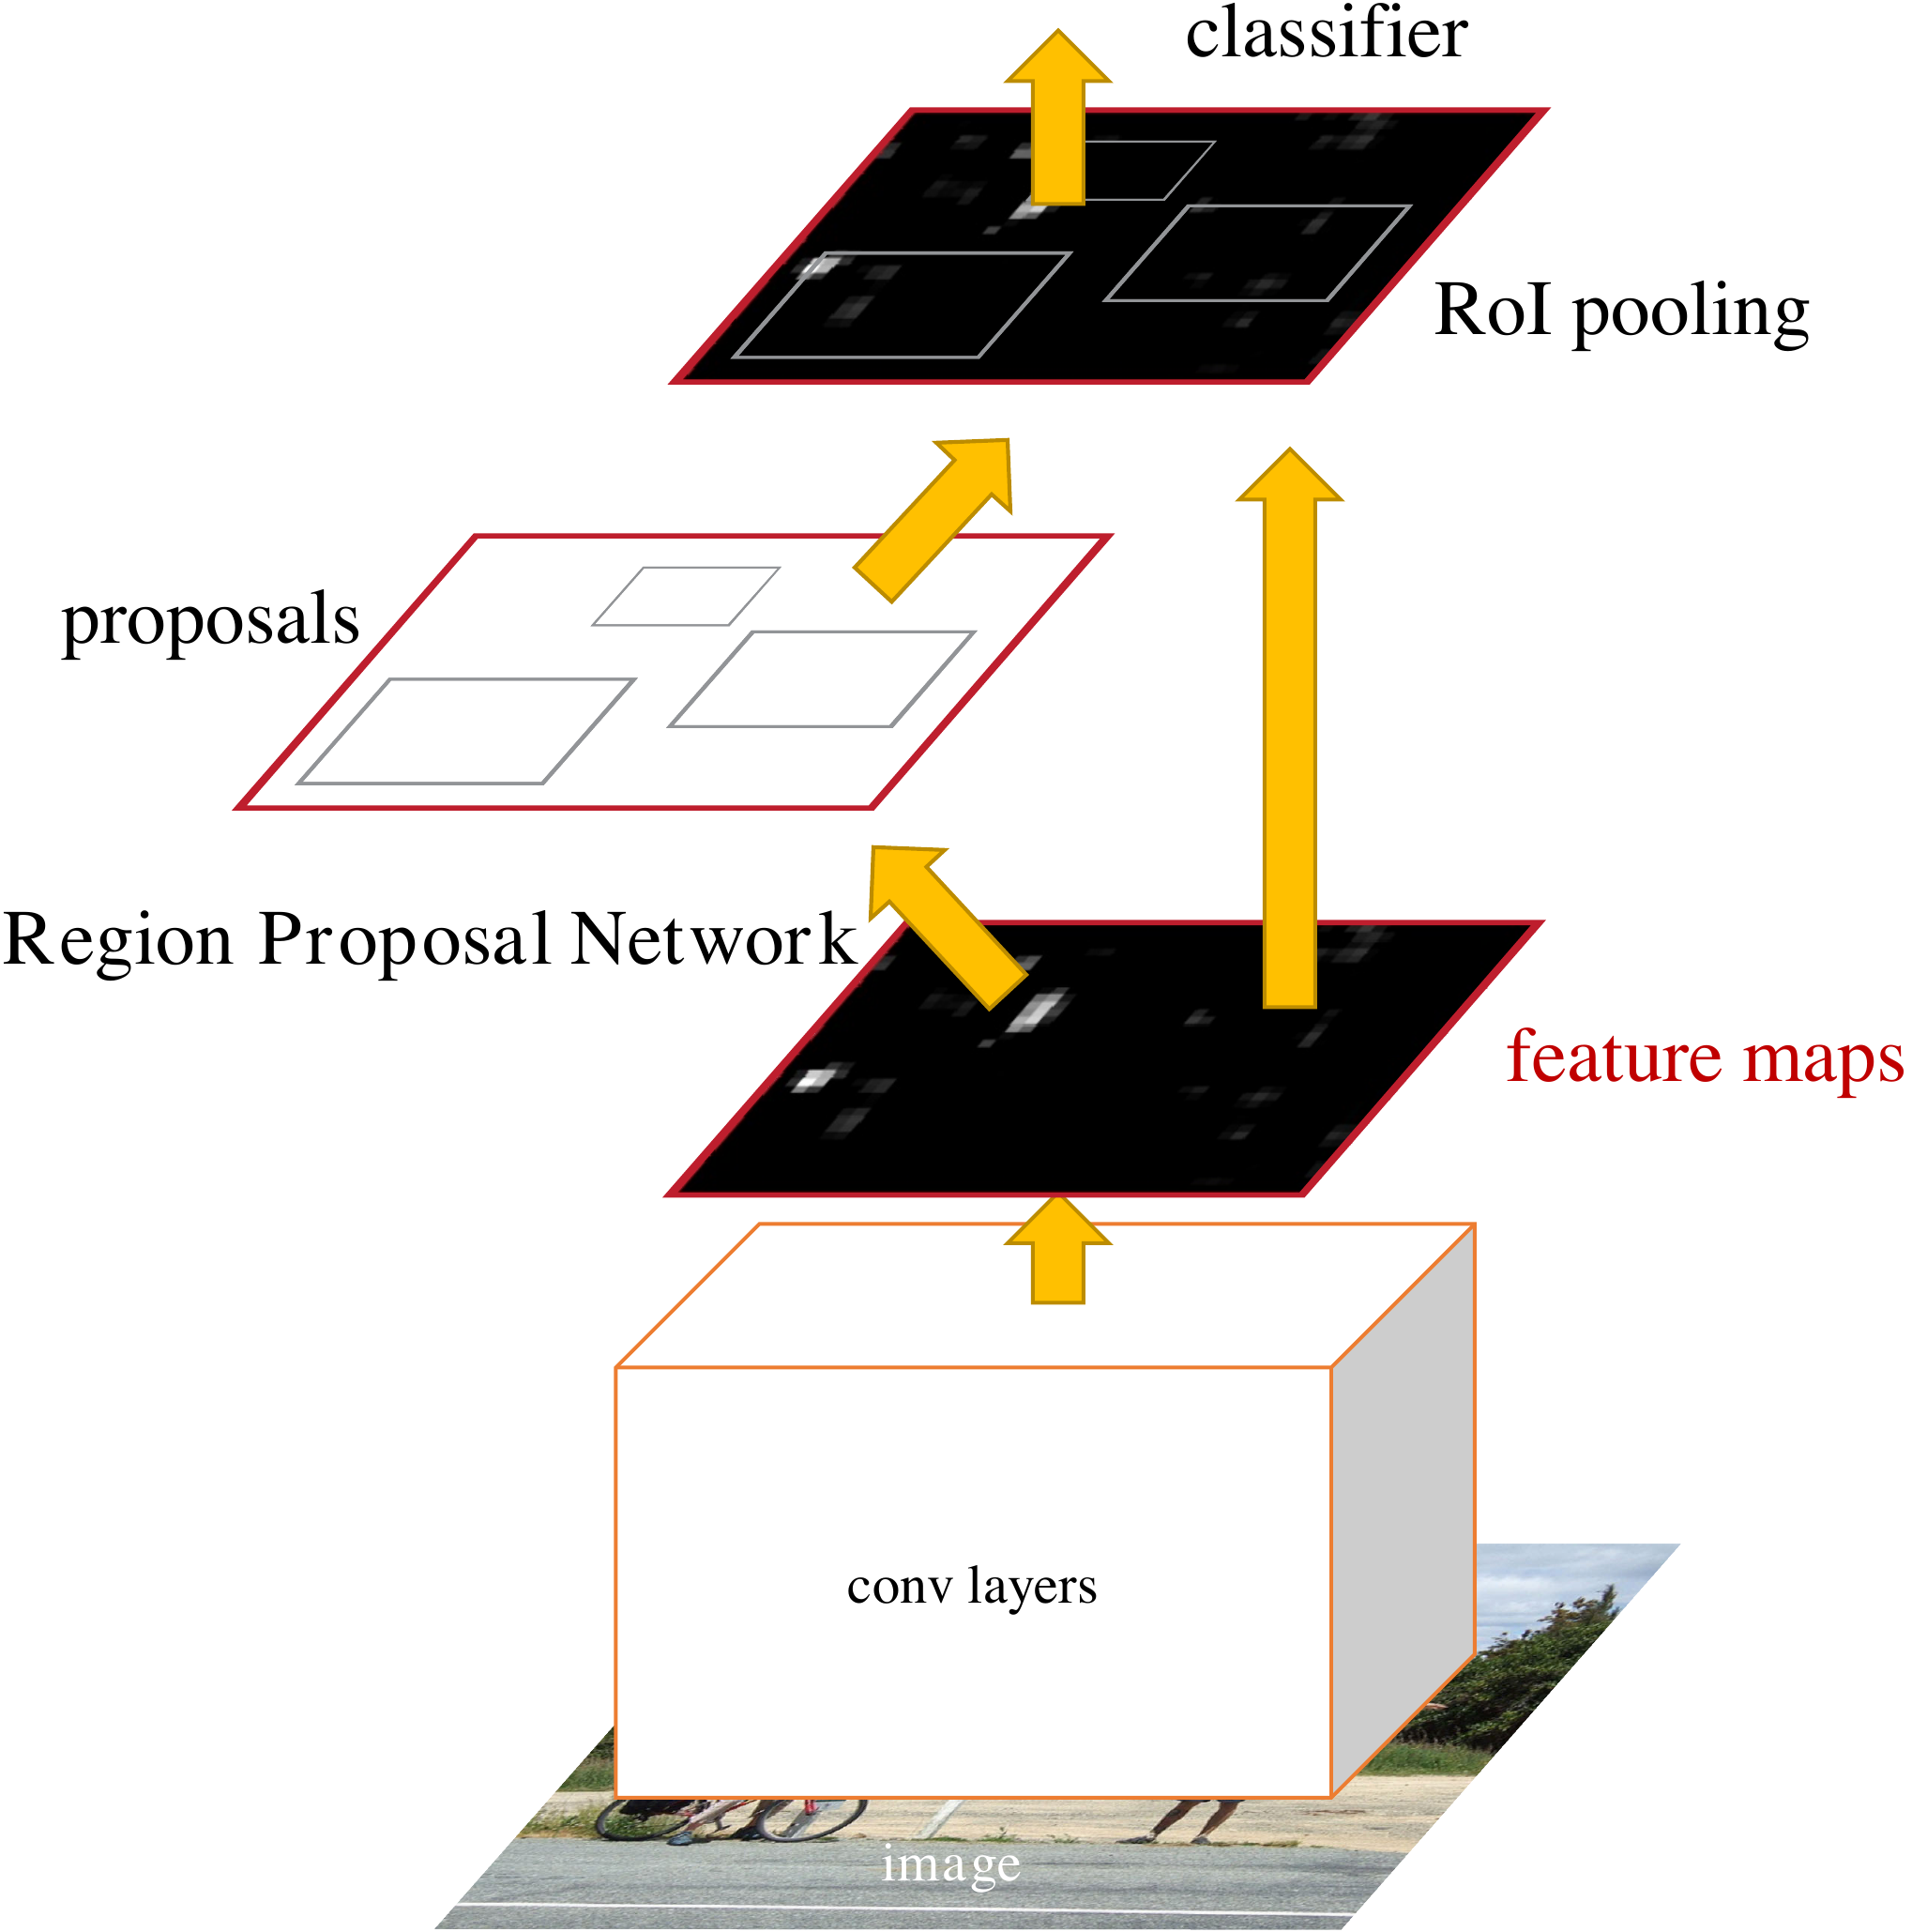
\includegraphics[width=0.5\textwidth]{../figure/fasterrcnn.png}
    \captionsetup{font=footnotesize}
    \bicaption{Faster RCNN 网络\cite{faster_rcnn}}{Faster RCNN Net}
    \label{fig:fasterrcnn}
\end{figure}

Faster R-CNN 的提出使得目标检测算法在高效性和准确性之间取得了更好的平衡。RPN 的引入大大加快了候选区域的生成速度,并且与整个检测网络共享卷积特征图,实现了端到端的训练和检测流程。这使得算法能够实时地处理图像数据,同时保持较高的检测精度,成为目前目标检测领域的主流算法之一,并且为后续的许多目标检测算法提供了基础架构。

Mask R-CNN 是在 Faster R-CNN 的基础上进行了扩展,主要用于同时进行目标检测和实例分割任务。Mask R-CNN 网络结构如图 \ref{fig:maskrcnn} 所示。在 Faster R-CNN 的目标检测框架基础上,Mask R-CNN 额外增加了一个分支网络用于预测每个目标实例的像素级分割掩码。具体来说,在 ROI Pooling 层之后,除了原来的全连接层用于分类和边界框回归外,增加了一个全卷积网络分支来预测目标的分割掩码。该分支网络对每个候选区域生成一个二值掩码,表示该区域内每个像素是否属于目标物体,从而实现对目标物体的精确分割。

\begin{figure}[htbp]
    \centering
    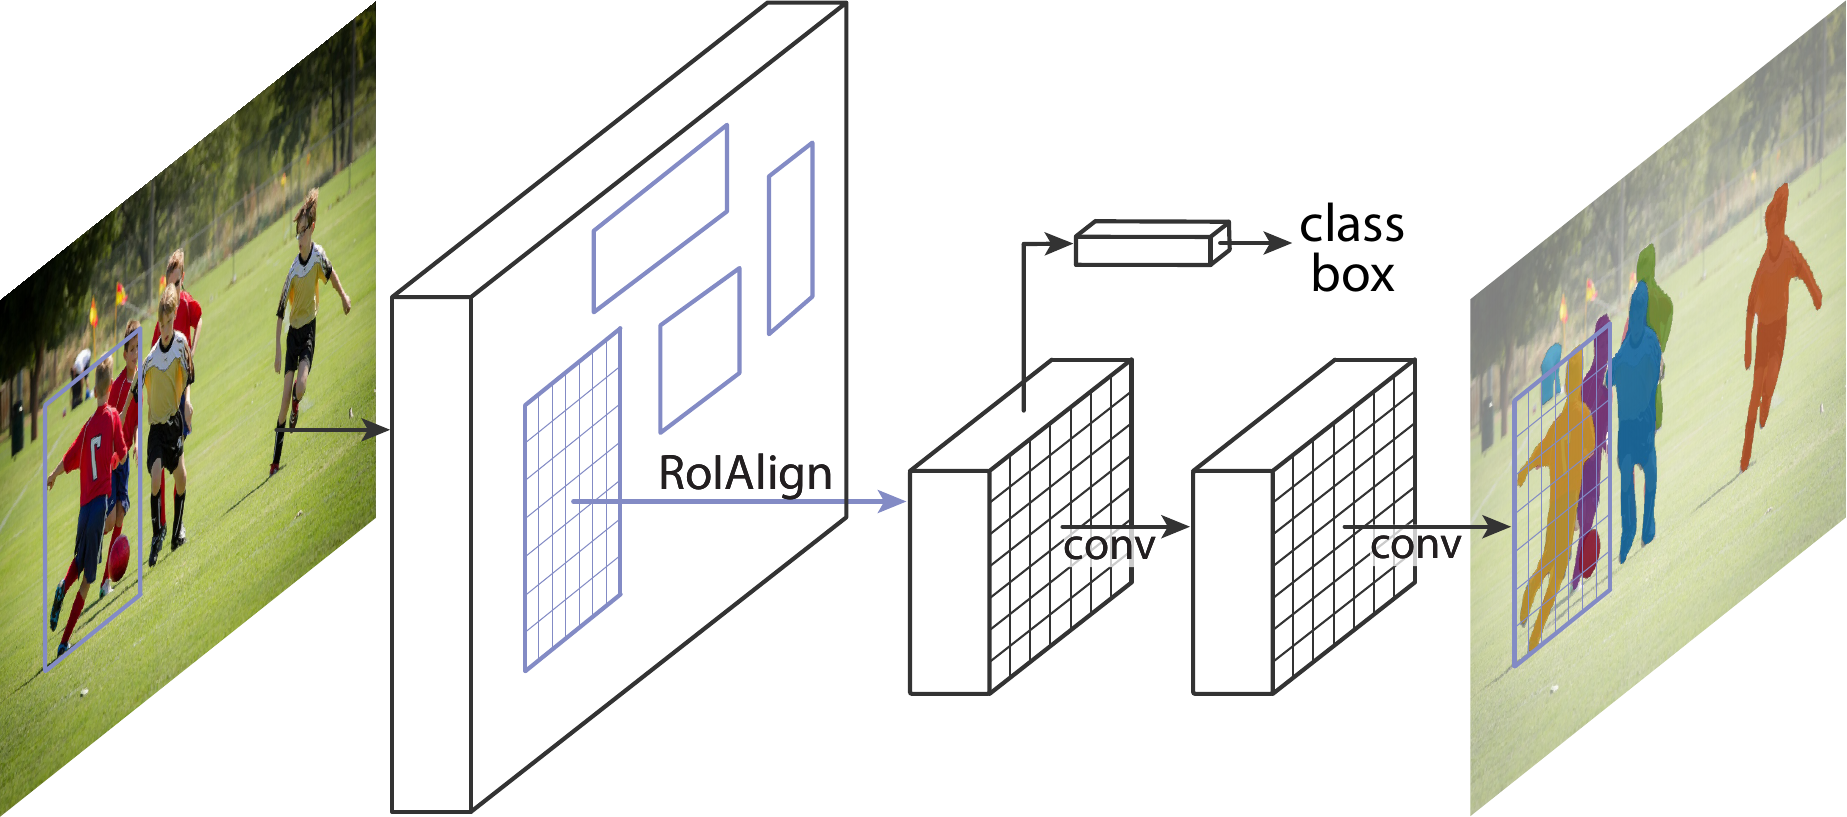
\includegraphics[width=0.7\textwidth]{../figure/maskrcnn.png}
    \captionsetup{font=footnotesize}
    \bicaption{Mask RCNN 网络\cite{mask_rcnn}}{Mask RCNN Net}
    \label{fig:maskrcnn}
\end{figure}

Mask R-CNN 在目标检测和实例分割领域都取得了优异的性能,它不仅能够准确地检测出图像中的目标类别和位置,还能对每个目标物体进行像素级别的分割,为更细粒度的图像理解和分析提供了支持。在诸如医学图像分析、自然场景理解等需要精确分割目标的应用场景中,Mask R-CNN 发挥了重要作用,并且推动了目标检测任务从单纯的边界框定位向更精细化的语义理解方向发展。

尽管在 Fast R-CNN 和 Faster R-CNN 等算法中对计算效率进行了优化,但由于双阶段算法涉及两个阶段的处理,包括候选区域的生成、特征提取、分类识别以及边界框回归等多个步骤,整体计算复杂度仍然较高。在处理高清图像或实时视频流时,可能难以满足实时性的要求,尤其是在资源受限的设备(如移动终端、嵌入式系统等)上,如何进一步降低算法的计算复杂度以实现高效实时的目标检测是一个重要的挑战。例如,在自动驾驶场景中,需要实时处理来自车辆摄像头的大量视频数据,以及时准确地识别道路上的车辆、行人、交通标志等目标,这对算法的实时性提出了极高的要求。

对于图像中的小目标物体,由于其在图像中占据的像素区域较少,特征信息相对有限,在双阶段目标检测算法中容易出现漏检或误检的情况。在候选区域生成阶段,小目标可能由于特征不明显而未被包含在候选区域中;在分类识别阶段,有限的特征信息也难以使模型准确地识别出小目标类别。例如在遥感图像中检测小型建筑物、在显微图像中检测细胞等小目标检测任务中,双阶段算法需要针对小目标的特点进行专门的优化和改进,如采用多层次特征融合策略、设计专门的小目标增强方法等,以提高对小目标的检测性能。

\subsubsection{单阶段目标检测算法}

单阶段目标检测算法摒弃了传统两阶段目标检测算法中先生成候选区域再进行分类识别的繁琐流程,而是将目标分类和定位任务同时进行,直接在图像上进行一次性的预测,从而大大提高了检测速度。其核心思想是将目标检测问题转化为一个端到端的回归问题,输入图像经过深度卷积神经网络的处理后,直接输出目标的类别概率和边界框坐标,这种一体化的处理方式使得单阶段目标检测算法具有较高的实时性和效率。

YOLO 系列\cite{yolov1, yolov2, yolov3, yolov4, yolov6, yolov7, yolov8, yolov9, yolov10, yolov11}算法作为单阶段目标检测算法的重要分支,基于深度学习的卷积神经网络构建其检测模型。卷积神经网络通过卷积层、池化层、激活函数等结构对图像进行特征提取和非线性变换,学习到图像的层次化特征表示。YOLO 网络结构如图 \ref{fig:yolov1} 所示。在 YOLO 算法中,网络将输入图像划分为多个大小相等的网格(grid cell),每个网格负责预测一定数量的边界框(bounding box)以及该边界框内包含目标物体的类别概率和边界框坐标。边界框的坐标通常包括边界框的中心坐标、宽度和高度等信息,而类别概率则表示该边界框内属于每个目标类别的可能性。

\begin{figure}[htbp]
    \centering
    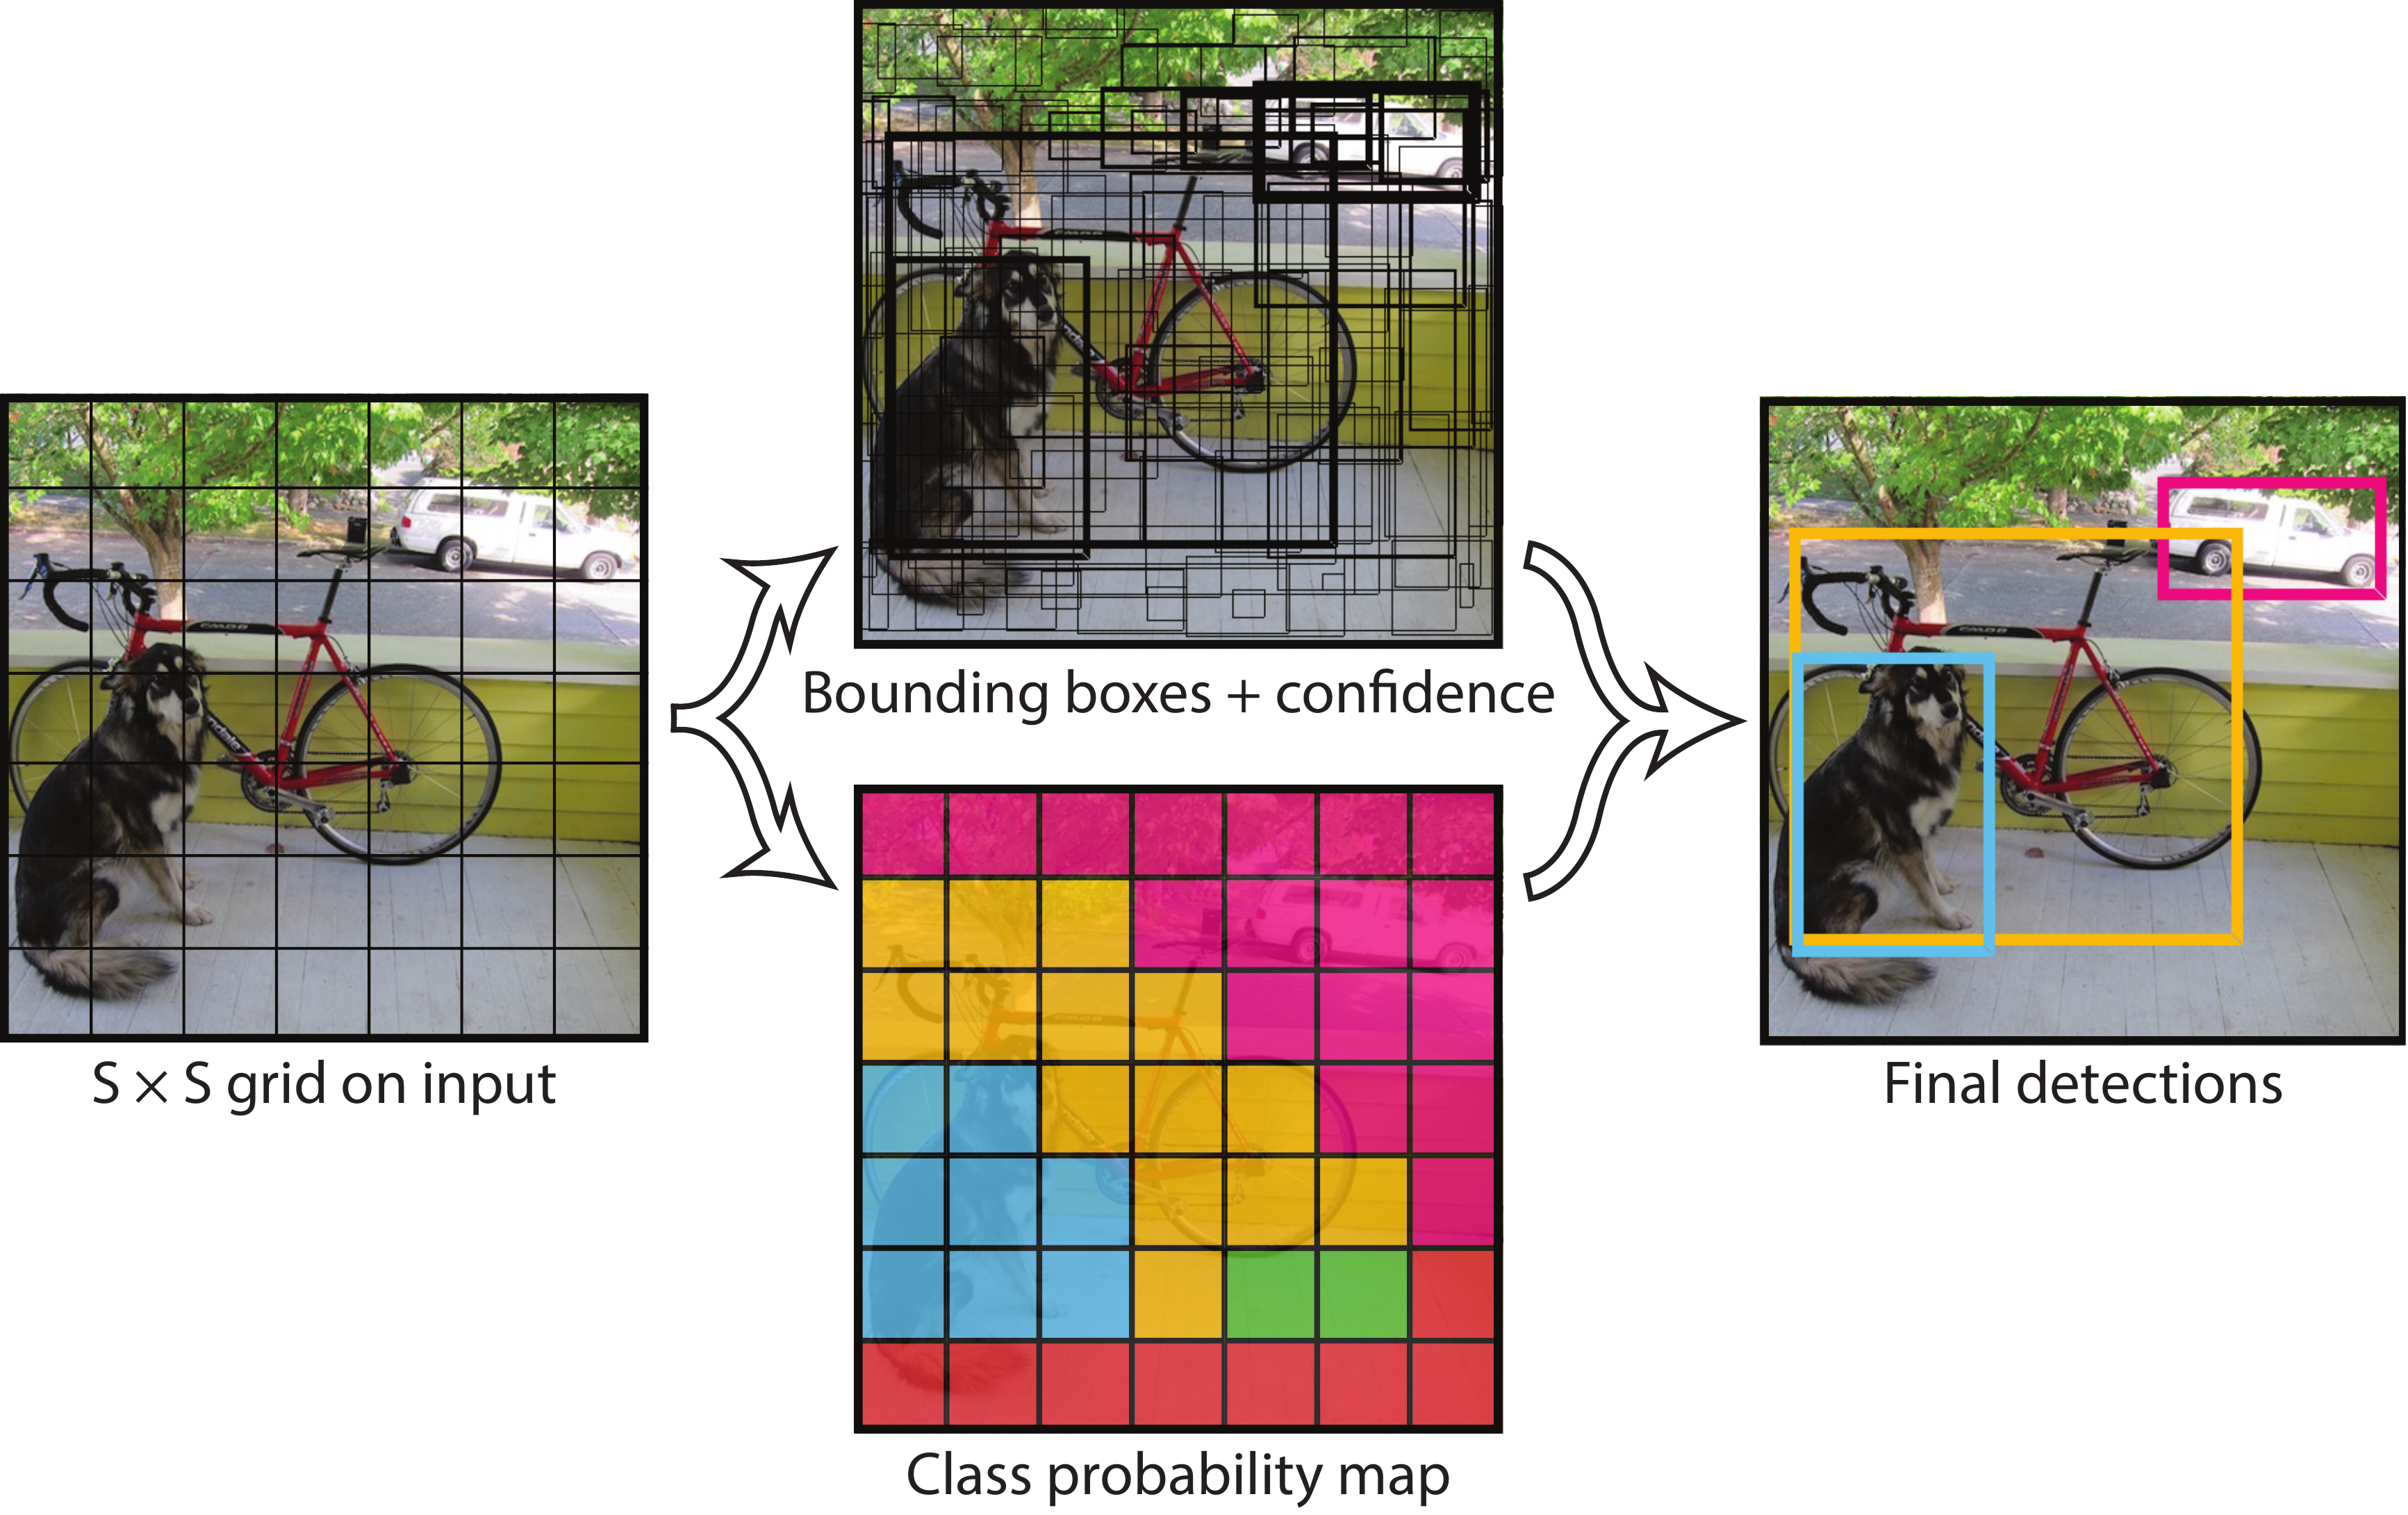
\includegraphics[width=0.7\textwidth]{../figure/yolov1.png}
    \captionsetup{font=footnotesize}
    \bicaption{YOLO 网络\cite{yolov1}}{YOLO Net}
    \label{fig:yolov1}
\end{figure}

在训练过程中,YOLO 系列算法采用监督学习的方式,利用标注有目标类别和边界框的训练数据对模型进行训练。通过定义损失函数,将预测的边界框坐标和类别概率与真实值之间的误差进行度量,并利用反向传播算法不断调整网络的参数,使得模型能够学习到准确的目标检测特征和知识,从而在测试时对新的图像进行快速、准确的目标检测。YOLOv4 网络结构如图 \ref{fig:yolov4} 所示。

\begin{figure}[htbp]
    \centering
    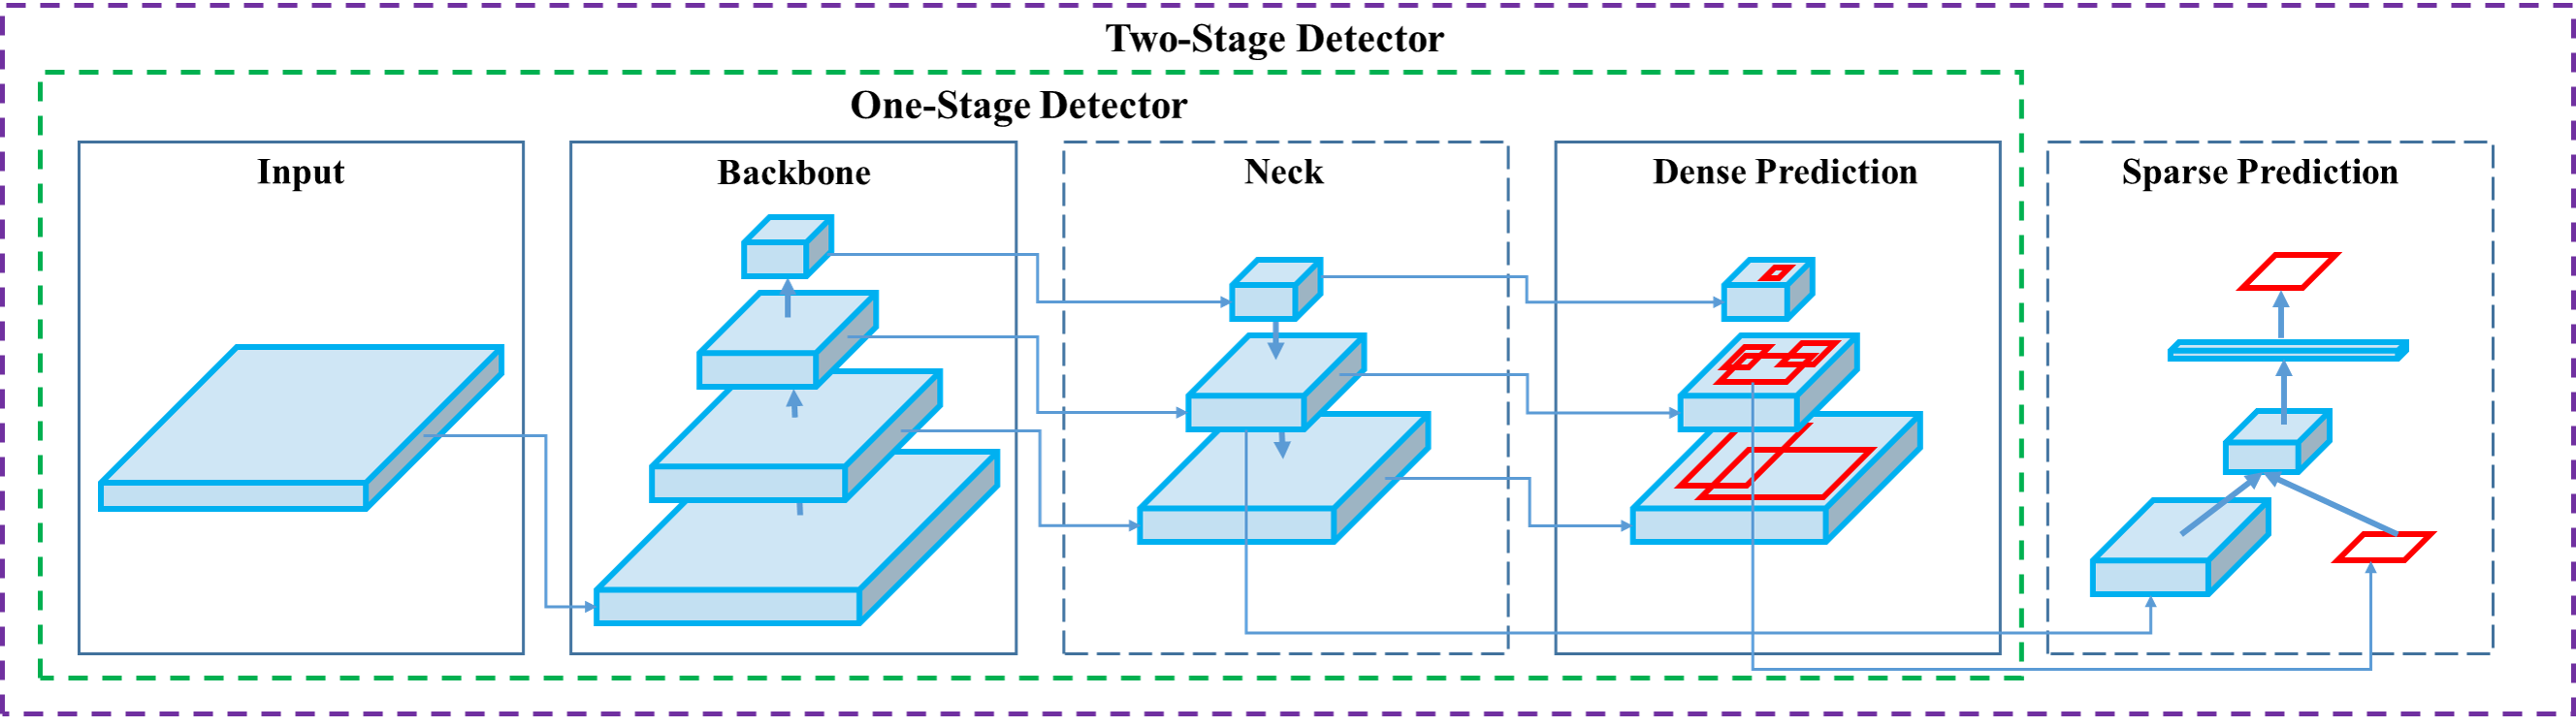
\includegraphics[width=0.8\textwidth]{../figure/yolov4.png}
    \captionsetup{font=footnotesize}
    \bicaption{YOLOv4 网络\cite{yolov4}}{YOLOv4 Net}
    \label{fig:yolov4}
\end{figure}

YOLOv5 以其简洁高效的特点,在工业界得到了广泛的应用和推广。它对 YOLO 系列算法进行了进一步的简化和优化,使其更易于部署和使用。
YOLOv5 在网络结构上进行了调整,采用了更少的参数量和计算量,同时保持了较高的检测精度。它引入了一种新的 PANet(Path Aggregation Network)结构\cite{pan},优化了特征融合的方式,使得特征信息能够更有效地在不同尺度之间传递和共享。此外,YOLOv5 还提供了多种不同规模的模型版本,以满足不同应用场景下对速度和精度的平衡需求。
YOLOv5 的出现大大降低了 YOLO 算法在实际工业应用中的部署门槛,使得更多的企业能够快速地将目标检测技术应用于产品开发和生产过程中,如智能安防、智能交通等领域。

在 YOLOv5 之后,YOLO 系列又相继推出了 YOLOv6、YOLOv7 和 YOLOv8 等版本。这些版本在前作的基础上不断进行改进和创新。
YOLOv6 专注于提高模型的效率和实时性,在移动端等资源受限设备上的表现尤为突出。它采用了更轻量化的网络结构和优化算法,进一步降低了模型的计算复杂度,同时通过一系列的优化技巧,如量化感知训练等,确保了模型在低精度硬件上的性能。
YOLOv7 则在速度和精度的平衡方面取得了新的突破,提出了一些新颖的架构设计和训练策略,使得模型能够在保持较高速度的同时,进一步提升检测精度,为高精度目标检测任务提供了更好的解决方案。
YOLOv8 改进的注意力机制和更先进的特征融合方法等。YOLOv8 在模型的易用性、灵活性以及性能方面都有显著的提升,能够适应各种不同的目标检测任务和应用场景。YOLOv8 网络结构如图 \ref{fig:yolov8} 所示。

\begin{figure}[htbp]
    \centering
    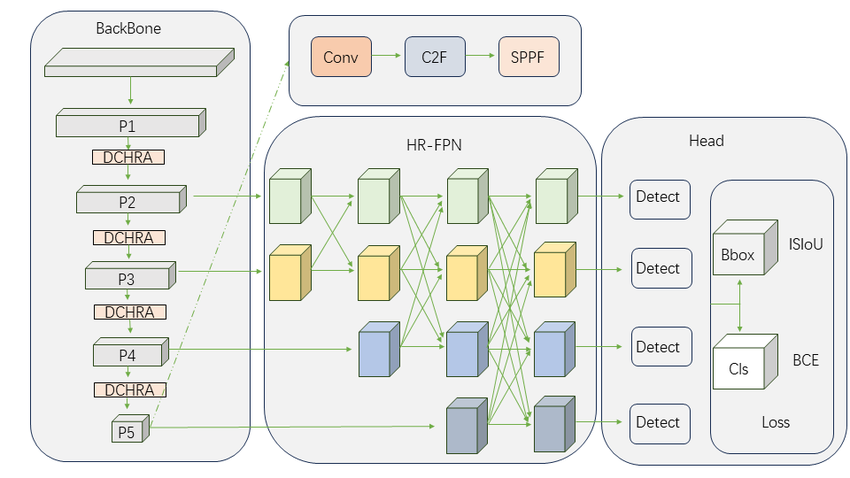
\includegraphics[width=0.8\textwidth]{../figure/yolov8.png}
    \captionsetup{font=footnotesize}
    \bicaption{YOLOv8 网络\cite{yolov8}}{YOLOv8 Net}
    \label{fig:yolov8}
\end{figure}

YOLO 系列算法作为单阶段目标检测算法的代表,其最大的优势在于能够实现实时、快速的目标检测。通过将目标检测任务转化为端到端的回归问题,省去了候选区域生成和特征提取的中间步骤,大大提高了检测速度。例如,YOLOv4 在常见的 GPU 设备上可以达到每秒数十帧甚至更高的检测速度,能够满足实时视频监控、自动驾驶等对实时性要求较高的应用场景的需求。

随着 YOLO 系列算法的不断演进,其检测精度也在不断提高。从 YOLOv1 到 YOLOv5,通过引入锚框机制、多尺度预测、改进的特征提取网络等技术手段,YOLO 系列算法在各种目标检测数据集上的平均精度均值(mAP)等性能指标上取得了显著的提升,能够准确地识别和定位图像中的目标物体,即使在复杂场景下也能保持较好的检测效果。

虽然 YOLO 系列算法在整体检测精度上取得了较好的成绩,但对于图像中的小目标物体,其检测精度仍然存在一定的提升空间。小目标物体由于在图像中占据的像素区域较少,特征信息有限,容易受到背景噪声和其他物体的干扰,导致 YOLO 算法在检测小目标时出现漏检或误检的情况。例如,在航拍图像中的行人检测、显微图像中的细胞检测等场景中,小目标检测的准确性仍然是 YOLO 系列算法需要进一步解决的难题。

在追求更高检测速度和精度的过程中,YOLO 系列算法需要在模型复杂度、计算资源消耗以及检测性能之间进行优化和平衡。随着模型深度和复杂度的增加,虽然检测精度可能会有所提高,但计算量和内存占用也会随之增大,这可能会导致算法在资源受限的设备上无法高效运行,甚至无法部署。因此,如何在保证检测性能的前提下,通过模型压缩、剪枝、量化等技术手段对 YOLO 系列算法进行优化,以适应不同硬件平台的性能要求,是当前 YOLO 系列算法发展面临的一个重要挑战。


\subsection{图像去雾还原的理论基础与算法}

\subsubsection{传统的图像去雾算法相关研究}

于晴朗天气下,场景中的物体光线能近乎直接、完整地抵达成像设备传感器,所获图像清晰且色彩精准。然雾天环境则截然不同,大气中的水汽凝结成微小水滴,悬浮于空气之中,其数量密度随雾浓度递增。当物体发出或反射的光线在传播途中,遭遇这些水滴时,便发生复杂的散射现象。
从光学层面而言,光线与雾粒子的相互作用遵循米氏散射理论。水滴尺寸与可见光波长相当,故米氏散射效应显著。入射光线在水滴表面发生散射,散射光强分布呈各向异性,部分光线偏离原传播方向,无法顺利抵达传感器。这就直接导致了场景中远处物体大量光线被散射损耗,成像时亮度信息弱化,图像整体暗淡且对比度严重下滑。不仅如此,不同波长光线散射程度有别,短波长的蓝光散射更为剧烈,使得雾天图像普遍呈现出偏蓝、偏灰的灰雾色调,色彩失真明显。

大气散射模型如图 \ref{dehaze} 所示。大气散射模型精准地数学化描述了雾天成像过程。其核心表达式为:
\begin{equation}
    \label{eq:haze2}
    I(x) = J(x)t(x)+A(1-t(x))
\end{equation}

公式\ref{eq:haze2}中,$I(x)$ 表示成像设备捕获的雾天图像某一点的观测强度;$J(x)$ 是该场景点在无雾状态下的真实场景辐射强度,蕴含着物体本来的颜色、纹理等关键信息;$t(x)$ 为大气透射率,衡量光线从场景点传播至传感器过程中,未被大气介质散射丢失的能量比例,其值介于 0 到 1 之间;$A$ 是大气光照,在均匀浓雾场景近似为常数,代表大气散射引入的背景光照强度,常呈现为灰白色调。
该模型直观展现了雾天图像退化根源:场景辐射光受大气阻碍衰减,同时大气散射光叠加其上。透射率 $t(x)$ 与大气光照 $A$ 成为模型两大关键参数,二者与雾浓度紧密关联且呈反向变化趋势。雾愈浓,透射率愈低,散射光干扰愈强,图像偏离真实场景愈远。

\begin{figure}[htbp]
    \centering
    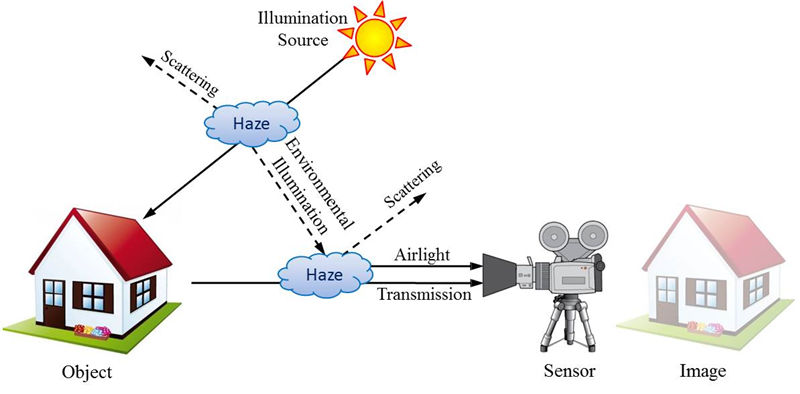
\includegraphics[width=0.8\textwidth]{../figure/dehaze.png}
    \captionsetup{font=footnotesize}
    \bicaption{大气散射模型\cite{cai2016dehazenet}}{Atmospheric Ejection Model.}
    \label{fig:dehaze}
\end{figure}

暗通道先验理论是图像去雾领域的重要突破。该理论基于在无雾自然图像的局部区域内,至少存在一种颜色通道(红、绿、蓝中的一个)具有非常低的像素强度这一观察结果。在无雾图像的局部区域中,往往存在一些没有被明亮光照直接照射到的暗区域,这些区域在某一颜色通道上的值会非常小,接近于零。在有雾图像中,由于雾的存在,这些暗区域的像素强度会被抬高,从而可以通过寻找图像中暗通道的最小值来估计大气光照,并进一步计算出传输系数。暗通道先预理论为图像去雾提供了一种有效的估计方法,具有计算效率高、对复杂场景适应性强等优点。但需要注意的是,暗通道先预在某些特定场景,如包含大面积亮白色物体或特殊光照条件的图像中,可能会出现估计误差,导致去雾效果不理想。

早期的基于物理模型的去雾算法主要依赖于对大气散射模型参数的手动估计,例如通过参考场景中的已知物体颜色或亮度来估计大气光照和传输系数。然而,手动估计参数的方法在实际应用中效率低下且准确性难以保证。随后,研究者们提出了一些基于物理模型的自动估计方法。例如,利用天空区域的特性来估计大气光照,假设天空区域的像素强度接近于大气光照强度,并通过图像分割技术提取天空区域进行估计。对于传输系数的估计,一些方法基于场景深度信息或散射系数的先验知识进行建模,如利用地形数据库或激光雷达测量数据来获取场景深度,进而计算传输系数。这类基于物理模型的方法在理论上有较强的物理意义,但在实际应用中往往对先验信息的依赖度较高,且计算复杂度较大,难以实时处理大规模图像数据。


图像处理相关理论也为图像去雾提供了支持。图像的对比度增强技术可以改善雾天图像的视觉效果,通过拉伸图像的灰度级范围,使图像中的暗细节更加清晰,但单纯的对比度增强并不能消除雾天图像中的散射光成分。图像的多尺度分析方法则可以从不同尺度上对图像进行分解和处理,有利于在去雾过程中同时保留图像的全局结构信息和局部细节特征。此外,图像的先验知识,如图像的边缘信息、纹理信息等,也可以作为约束条件融入到去雾算法中,以提高去雾的精度和质量。

基于图像处理的去雾算法不直接依赖于大气散射模型,而是通过对图像的像素强度、颜色分布、纹理等特征进行分析和处理来实现去雾效果。常见的基于图像处理的去雾算法包括基于图像对比度增强的方法、基于滤波的方法等。

基于图像对比度增强的方法通过对图像的灰度级或颜色通道进行拉伸、均衡化等操作,来提高图像的对比度,从而改善雾天图像的能见度。例如,直方图均衡化技术是一种简单而常用的对比度增强方法,它通过调整图像像素的分布,使图像的灰度级范围更加均匀,从而增强图像的对比度。然而,单纯的对比度增强方法可能会导致图像的色彩失真,且无法有效去除图像中的散射光成分。

基于滤波的方法则利用滤波器对图像进行处理,以提取图像中的有用信息并抑制雾的影响。高通滤波器可以突出图像中的高频细节信息,如边缘、纹理等,而低通滤波器则可以平滑图像中的噪声和模糊成分。一些去雾算法将高通滤波和低通滤波相结合,通过在不同频域上对图像进行处理来实现去雾效果。例如,通过高通滤波提取图像的细节信息,然后将其与经过低通滤波处理后的图像进行融合,以恢复出清晰的图像。此外,还有一些基于自适应滤波的去雾方法,可以根据图像局部区域的特性自动调整滤波器的参数,以更好地适应不同场景下的去雾需求。但基于滤波的去雾算法也可能存在一些问题,如滤波器的设计和参数选择对去雾效果影响较大,且在处理复杂图像时可能会出现伪影等现象。

传统图像去雾算法在理论和实践中都取得了一定的成果,但它们也存在一些局限性。基于物理模型的方法对先验信息的依赖性强,且计算复杂度较高;基于图像处理的方法虽然计算效率相对较高,但在去雾精度和效果上可能不如基于物理模型的方法。随着计算机视觉技术和机器学习技术的不断发展,新的图像去雾算法不断涌现,这些新算法在一定程度上克服了传统算法的不足,为图像去雾技术的发展带来了新的机遇和挑战。

\subsubsection{基于深度学习的图像去雾算法相关研究}

深度学习技术以其强大的特征自动学习能力,在图像去雾领域展现出独特的优势。传统的图像去雾方法往往依赖于人工设计的特征提取和先验知识,处理复杂场景时存在局限性。而深度学习模型,尤其是卷积神经网络(CNN),能够自动从大量带有雾和无雾的图像数据中学习到丰富的特征表示。这些特征涵盖了从低层的纹理、边缘信息到高层的语义信息,使得模型在面对多样化的雾天图像时,能够更精准地理解场景内容和雾的影响模式。例如,在城市街景图像去雾中,深度学习模型可以自动识别出建筑物、道路、车辆等不同物体的特征,并针对性地进行去雾处理,恢复出清晰的图像结构。此外,深度学习模型具有良好的泛化能力,经过充分训练后,能够在不同光照条件、不同雾浓度以及不同场景类型的图像上保持相对稳定的去雾效果。

端到端的卷积神经网络去雾算法以雾天图像作为输入,直接输出对应的无雾图像。其核心在于构建一个深度卷积神经网络模型,该模型通过大量的带有雾和无雾图像对进行训练,自动学习雾天图像与无雾图像之间的复杂非线性映射关系。在网络训练过程中,卷积神经网络的多层卷积结构能够自动提取图像的特征,从低层的边缘、纹理等基本特征到高层的语义特征。这些特征对于理解和恢复图像中的场景内容以及去除雾的影响至关重要。例如,卷积层中的卷积核可以看作是特征提取器,通过与图像进行卷积操作,生成特征图,突出图像中与去雾相关的特定模式和结构。池化层则用于降低特征图的维度,减少计算量的同时保留关键特征信息,增强模型对图像尺度变化的适应性。

在网络的反向传播过程中,通过定义合适的损失函数,如均方误差损失(MSE)或结构相似性损失(SSIM),来衡量生成的无雾图像与真实无雾图像之间的差异。模型根据损失函数的反馈,自动调整网络中的权重参数,使得网络不断学习和优化特征提取与映射能力,最终达到准确去雾的目的。

DehazeNet\cite{cai2016dehazenet} 是早期具有代表性的基于卷积神经网络的端到端去雾算法。DehazeNet 网络结构如图 \ref{fig:dehazenet} 所示。它采用了多层卷积结构,专门设计用于估计大气散射模型中的传输系数。DehazeNet 的网络结构相对简单,但有效。它通过三个卷积层逐步提取雾天图像的特征,并利用这些特征来估计传输系数,进而根据大气散射模型恢复出无雾图像。该算法首次将深度学习技术应用于图像去雾领域,并取得了一定的成果,在一些常见的图像去雾数据集上表现出了较好的性能,为后续基于深度学习的去雾研究奠定了基础。然而,DehazeNet 也存在一些局限性,例如模型参数较多,导致计算复杂度较高,训练和测试速度较慢,在处理大规模图像数据时效率较低。

\begin{figure}[htbp]
    \centering
    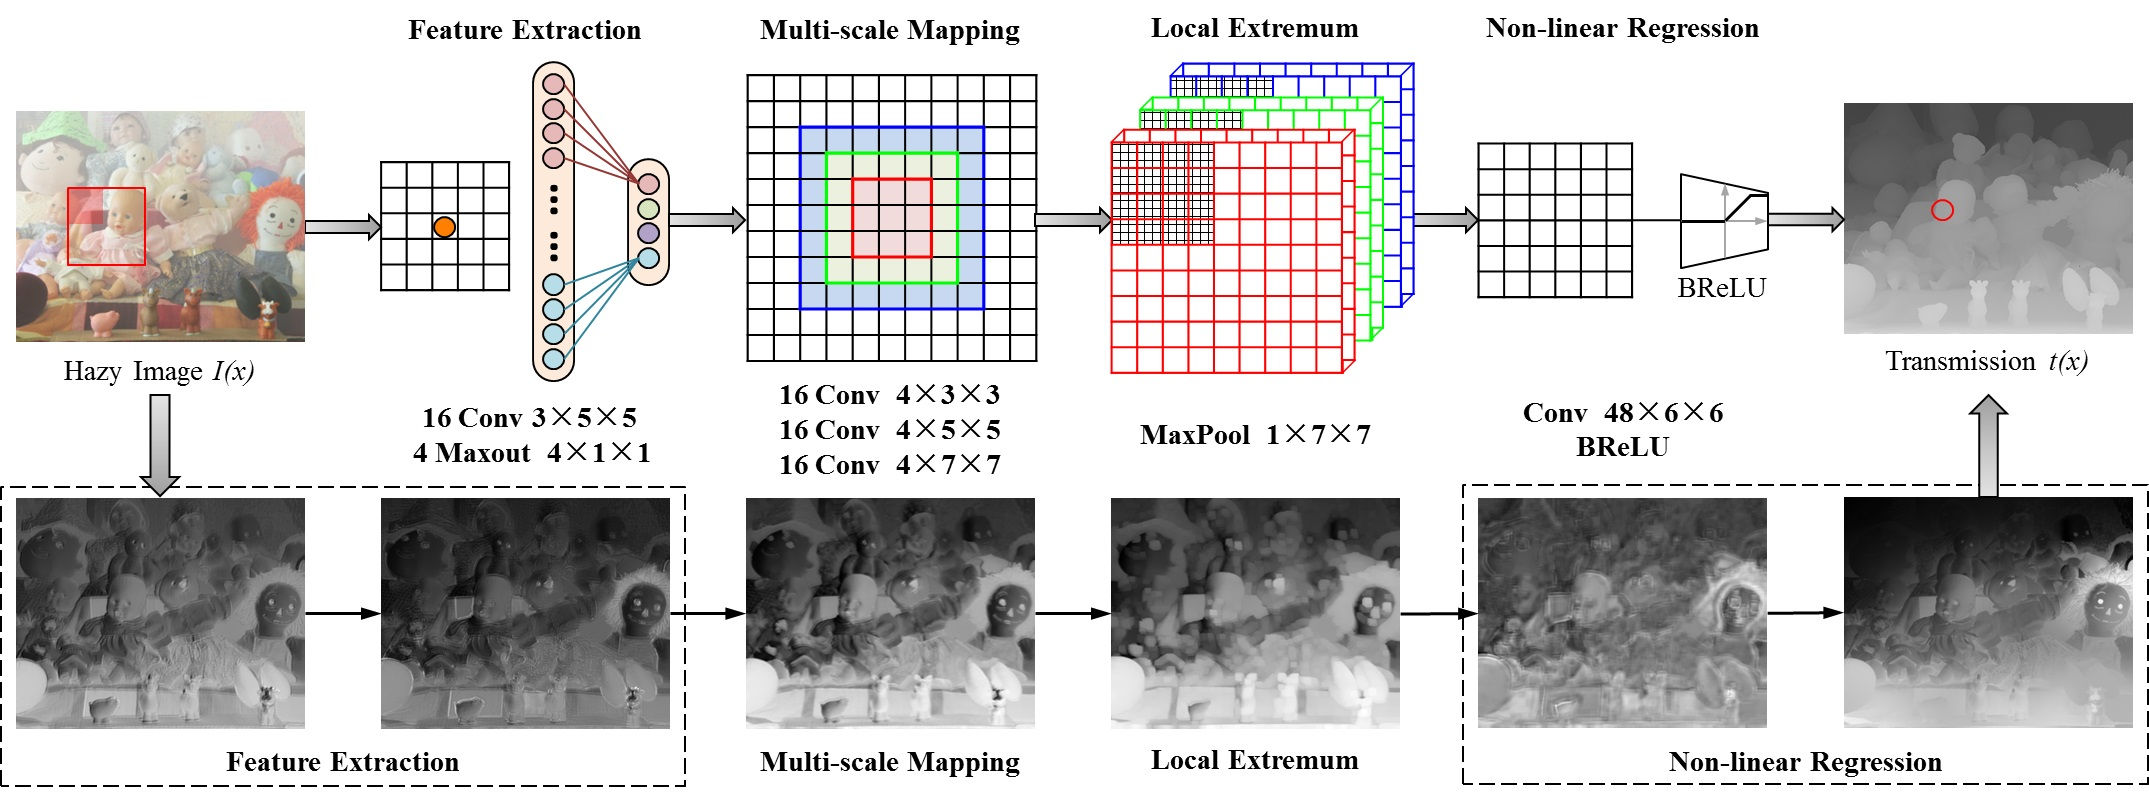
\includegraphics[width=0.9\textwidth]{../figure/hazenet.png}
    \captionsetup{font=footnotesize}
    \bicaption{DeHaze 网络\cite{cai2016dehazenet}}{DeHaze Net}
    \label{fig:dehazenet}
\end{figure}

为了解决 DehazeNet 等早期算法存在的问题,AOD-Net 应运而生。AOD-Net 提出了一种更紧凑的网络架构,将大气散射模型的逆过程融入到网络中,能够同时估计大气光照和传输系数。AOD-Net 网络结构如图 \ref{fig:aodnet} 所示。其网络结构主要包括一个编码器和一个解码器。编码器部分通过卷积层和池化层提取图像的多尺度特征,逐步降低特征图的空间维度,同时增加通道数,提取更抽象的特征。解码器部分则通过反卷积层或上采样层将编码器提取的特征逐步恢复到与输入图像相同的空间维度,生成对应的无雾图像。AOD-Net 引入了残差学习思想,在网络的每一层都学习输入与输出之间的残差,使得网络更容易训练,能够更快地收敛,并且有效地缓解了梯度消失问题。实验表明,AOD-Net 在多个公开数据集上的去雾性能优于以往的传统方法和一些早期的深度学习方法,能够生成更清晰、自然的无雾图像,并且在计算速度上有显著提升,具有较好的实时性。

\begin{figure}[ht]
    \centering
    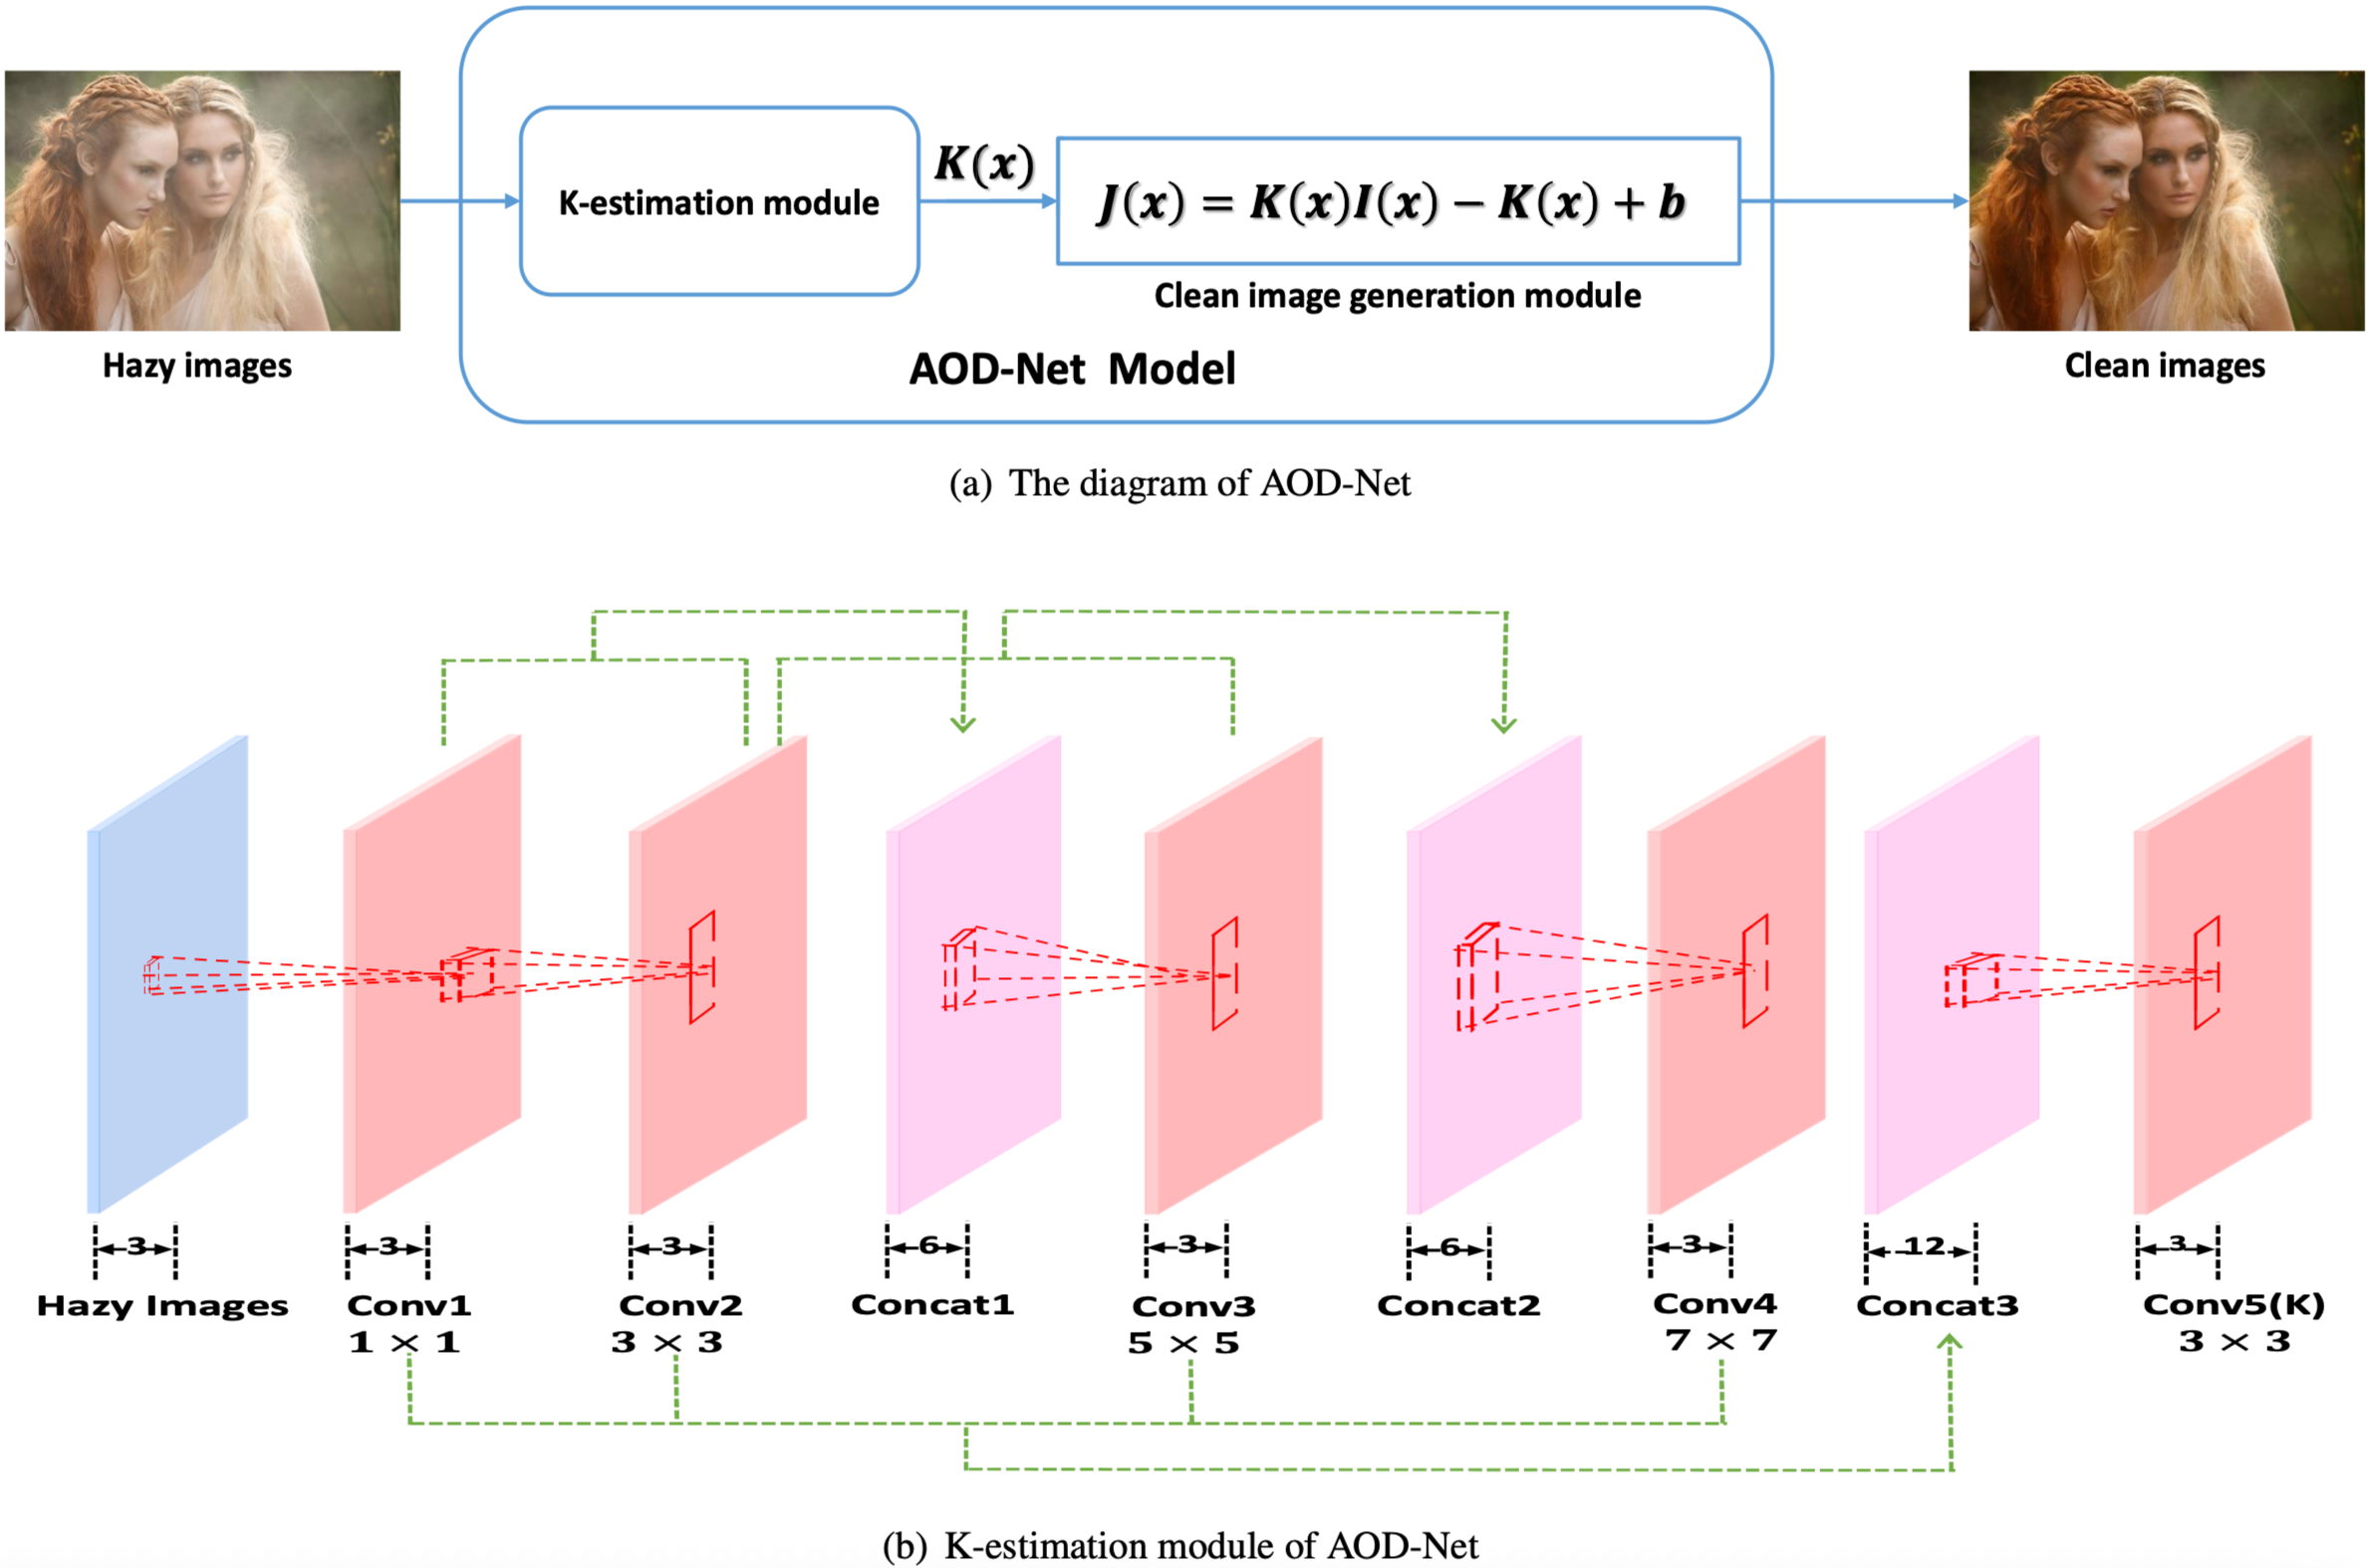
\includegraphics[width=0.8\textwidth]{../figure/aodnet.png}
    \captionsetup{font=footnotesize}
    \bicaption{AOD-Net 网络\cite{li2017aod}}{AOD-Net}
    \label{fig:aodnet}
\end{figure}

MSCNN\cite{zeng2017multi} 是另一种经典的基于卷积神经网络的端到端去雾算法。MSCNN 网络结构如图 \ref{fig:mscnn} 所示。它创新性地采用了多尺度网络结构来解决图像去雾中的细节恢复问题。MSCNN 包括两个子网络:一个全局子网络和一个局部子网络。全局子网络用于捕捉图像中的大尺度特征,如整体场景的结构和大气光照分布等;局部子网络则侧重于提取图像中的小尺度特征,如物体的边缘和纹理细节等。通过将全局和局部子网络的输出进行融合,MSCNN 能够更准确地恢复出无雾图像中的细节信息,避免了单一尺度网络可能出现的细节丢失或模糊问题。多尺度网络结构使得该算法在处理不同复杂度和不同分辨率的图像时具有更强的适应性和灵活性。例如,在处理包含精细纹理(如树叶、毛发等)的图像时,MSCNN 能够更好地保留这些细节,使去雾后的图像更加生动逼真。不过,MSCNN 的多尺度网络结构也导致其模型参数量和计算量相对较大,在实际应用中对硬件设备的计算能力有一定的要求。

\begin{figure}[ht]
    \centering
    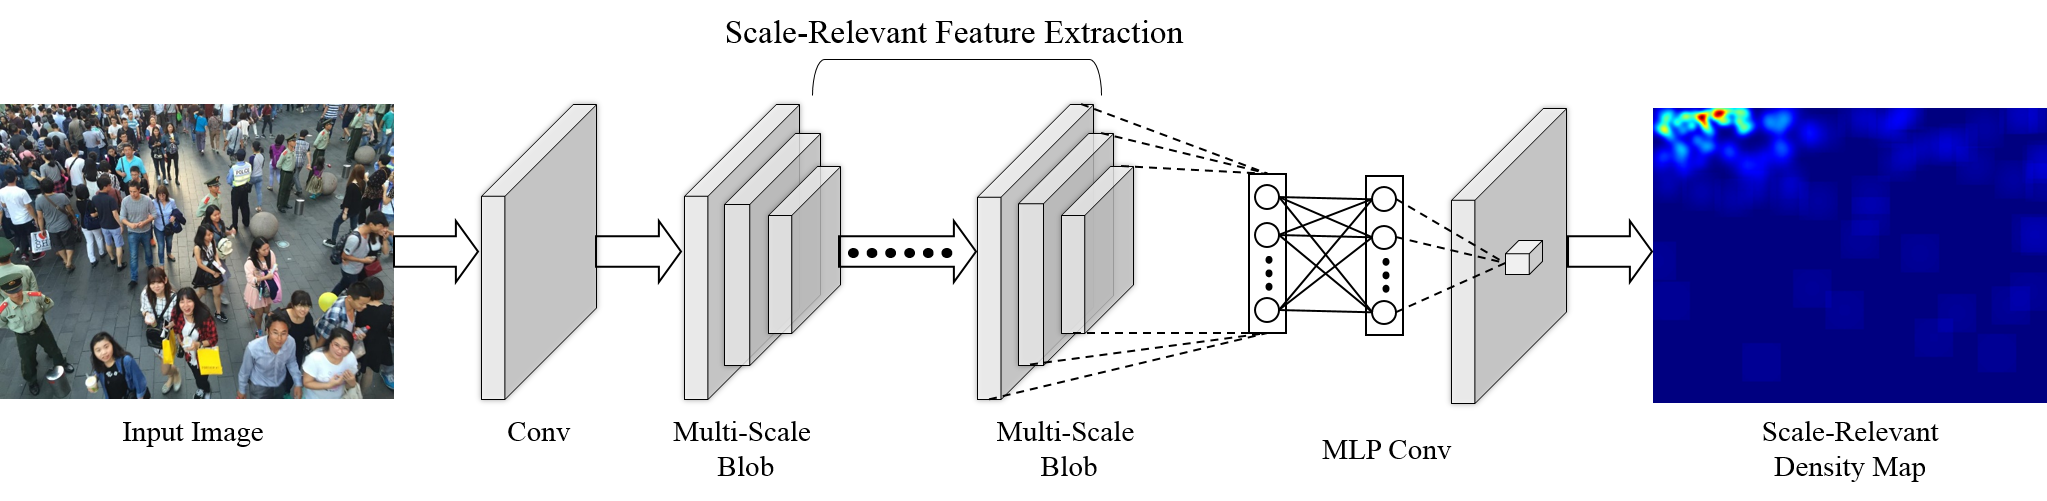
\includegraphics[width=0.9\textwidth]{../figure/mscnn.png}
    \captionsetup{font=footnotesize}
    \bicaption{MSCNN 网络\cite{zeng2017multi}}{MSCNN Net}
    \label{fig:mscnn}
\end{figure}

基于卷积神经网络的端到端去雾算法具有显著的优势。首先,它们能够自动学习图像中的复杂特征,不需要人工设计特征提取方法,大大提高了去雾算法的自动化程度和适应性。通过大量的数据训练,模型可以学习到不同类型场景、不同光照条件和不同雾浓度下的去雾模式,从而对各种雾天图像都能实现较好的去雾效果。其次,端到端的网络结构使得整个去雾过程更加简洁高效,避免了传统去雾方法中复杂的中间步骤和参数调整,减少了人工干预和计算错误的可能性。此外,随着硬件技术的发展,如图形处理器(GPU)的计算能力不断提升,这些基于卷积神经网络的端到端去雾算法能够实现较快的训练和测试速度,满足一些实时性要求较高的应用场景,如自动驾驶中的图像去雾辅助系统等。

然而,这类算法也存在一些局限性。首先,对训练数据的依赖程度较高。为了训练出性能良好的模型,需要大量的带有雾和无雾对应关系的图像数据。但在实际中,获取高质量的成对图像数据较为困难,因为很难保证在相同的场景和条件下分别拍摄到雾天和无雾的图像,并且图像的拍摄角度、光照强度等因素也可能存在差异,这会影响模型的训练效果和泛化能力。其次,模型的可解释性较差。由于卷积神经网络是复杂的黑盒模型,很难直观地理解网络内部是如何提取特征以及进行去雾映射的,这在一定程度上限制了对算法性能优化的深入研究和对特殊场景去雾效果的预测与改进。再者,一些端到端去雾算法在处理一些特殊场景或低质量的雾天图像时,可能会出现去雾效果不理想的情况,如图像出现伪影、颜色失真或细节过度增强等,这需要进一步优化网络结构和训练策略来解决。

生成对抗网络(GAN)\cite{gan}由生成器和判别器两部分组成,二者相互对抗、共同训练。生成器旨在生成逼真的无雾图像,而判别器则负责区分生成的无雾图像和真实的无雾图像。通过不断地对抗训练,生成器逐步学习到真实的图像数据分布,从而能够生成高质量的无雾图像,判别器也在这个过程中不断提升其判别能力。这种对抗训练机制使得 GAN 在图像生成和图像到图像的转换任务中展现出强大的性能,为图像去雾领域带来了新的思路和突破。

DehazeGAN\cite{raj2020single} 是较早将 GAN 引入图像去雾领域的算法之一。DehazeGAN 网络结构如图 \ref{fig:dehazegan} 所示。它通过构建生成器和判别器网络结构,利用对抗训练的思想来实现图像去雾。生成器采用编码器 - 解码器结构,编码器部分提取雾天图像的特征,解码器部分则根据提取的特征生成对应的无雾图像。判别器则是一个卷积神经网络,用于判断输入的图像是否为真实的无雾图像。在训练过程中,生成器和判别器不断更新参数,彼此竞争,使得生成器生成的无雾图像在视觉效果上更加逼真。DehazeGAN 在一定程度上提高了图像去雾的效果,能够生成较为自然的无雾图像,并且在一些简单的雾天图像场景下表现良好。然而,该算法也存在一些不足之处,例如在处理复杂场景时,生成的无雾图像可能会出现一些伪影,且对训练数据的质量和数量较为敏感,当训练数据不足或质量较差时,模型的性能会受到较大影响。

\begin{figure}[ht]
    \centering
    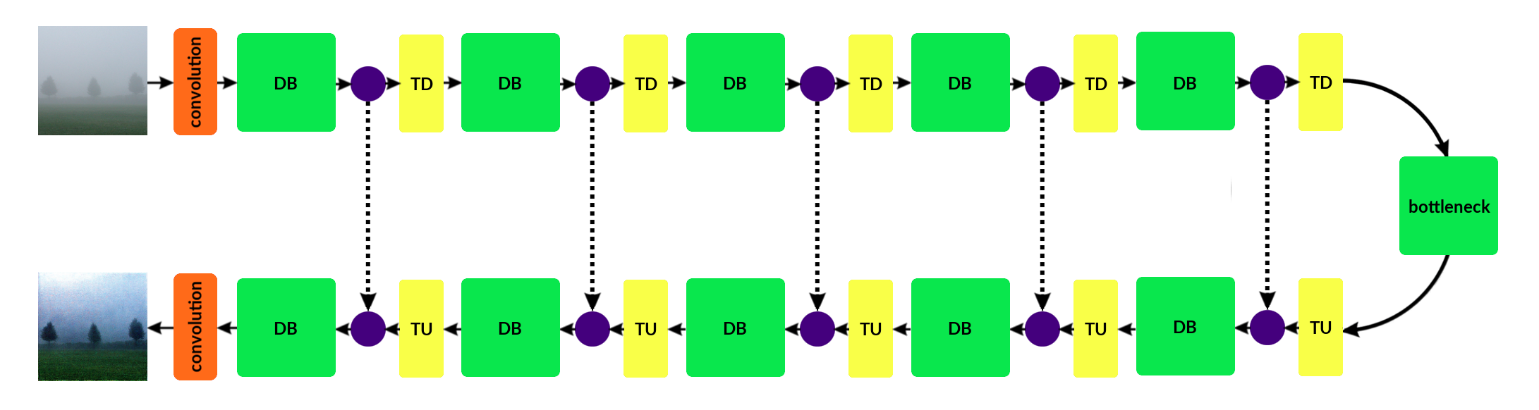
\includegraphics[width=0.8\textwidth]{../figure/dehazeGANG.png}
    \\
    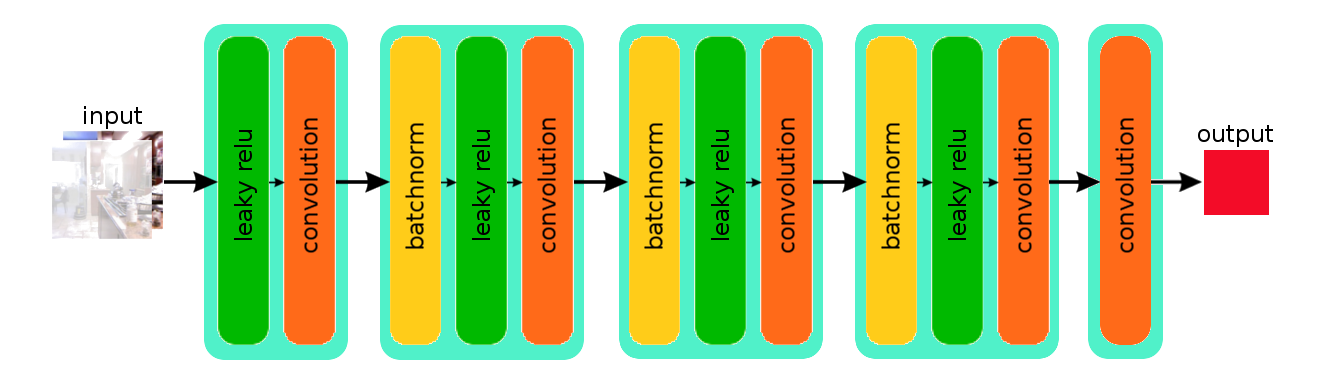
\includegraphics[width=0.8\textwidth]{../figure/dehazeGAND.png}
    \captionsetup{font=footnotesize}
    \bicaption{DehazeGAN 网络\cite{raj2020single}}{DehazeGAN Net}
    \label{fig:dehazegan}
\end{figure}

为了克服 DehazeGAN 等算法存在的问题,CycleDehazeGAN 被提出\cite{cgan}。CycleDehazeGAN 网络结构如图 \ref{fig:cycledehaze} 所示。该算法引入了循环一致性损失函数,通过构建两个生成器和两个判别器,实现从雾天图像到无雾图像以及从无雾图像到雾天图像的双向转换,并利用循环一致性约束来保证图像在转换过程中的信息完整性和一致性。具体来说,一个生成器将雾天图像转换为无雾图像,另一个生成器将无雾图像转换为雾天图像,同时两个判别器分别对转换后的无雾图像和雾天图像进行判别。循环一致性损失函数确保了经过双向转换后的图像与原始图像在内容和结构上的一致性,从而有效地避免了图像在转换过程中出现信息丢失或伪影等问题。CycleDehazeGAN 在处理复杂场景和多样化数据时具有更好的稳定性和鲁棒性,能够生成更高质量的无雾图像,并且在无监督学习环境下也能取得较好的去雾效果,扩大了其应用范围。

\begin{figure}[ht]
    \centering
    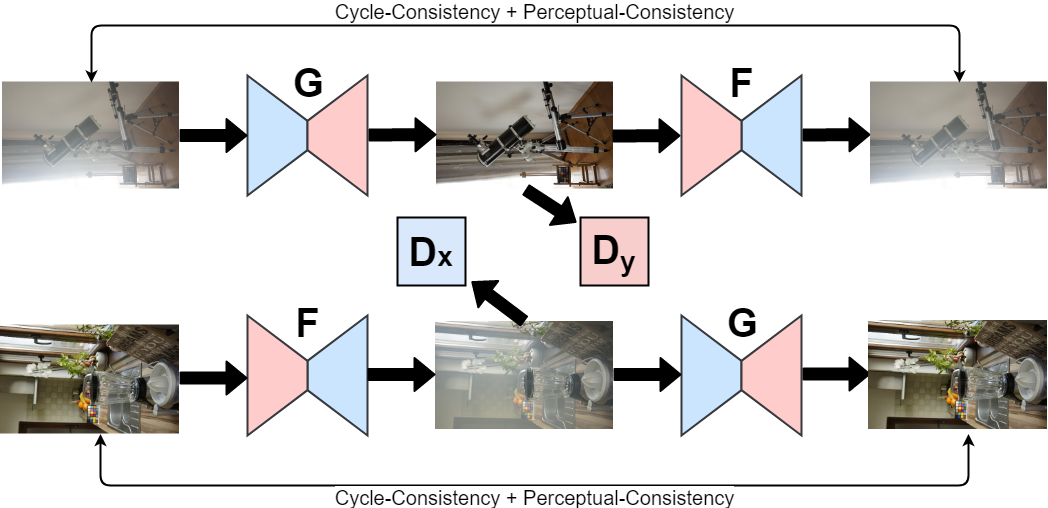
\includegraphics[width=0.7\textwidth]{../figure/Cycle-Dehaze.png}
    \captionsetup{font=footnotesize}
    \bicaption{CycleDehazeGAN 网络\cite{cgan}}{CycleDehazeGAN Net}
    \label{fig:cycledehaze}
\end{figure}

基于 GAN 的图像去雾算法具有显著的优势。首先,GAN 的对抗训练机制能够使生成器生成的无雾图像在视觉效果上更加逼真,更好地保留了图像的细节和纹理信息,避免了传统去雾方法可能出现的过度平滑或细节丢失等问题。例如,在去雾后的图像中,物体的边缘更加清晰锐利,表面的纹理更加丰富自然,这有助于提高图像的视觉质量和后续计算机视觉任务的准确性。其次,GAN 方法能够实现无监督或弱监督学习,在一定程度上缓解了获取大量成对雾天图像和无雾图像数据困难的问题,扩大了算法的应用范围和实用性,可以利用更多的未标注数据进行训练,提高了模型的泛化能力。再者,GAN 的灵活架构使得研究人员可以根据不同的需求和场景对网络结构进行定制和改进,例如引入多尺度结构、注意力机制等,以进一步提升去雾效果和适应性。


\subsection{目标检测算法的评价指标}

\subsubsection{基础指标}

准确率是指在所有被预测为正样本(即检测到目标)的结果中,实际为真阳性(True Positive)的比例。其计算公式如下:
\begin{equation}
    \label{eq:p}
    P = \frac{TP}{TP+FP}
\end{equation}

公式 \ref{eq:p} 中,$TP$(True Positive)代表正确检测到的目标数量,$FP$(False Positive)表示错误检测到的目标数量。准确率越高,表明算法在预测目标存在时的可信度越高,对虚假目标的误判越少。例如,在安防视频监控的目标检测场景中,较低的准确率可能导致大量误报,增加人工审核工作量,而高准确率的算法能有效减少此类干扰,精准定位真正可疑目标。


召回率衡量的是算法在所有真实存在的目标中,能正确检测出的比例。计算公式为:
\begin{equation}
    \label{eq:r}
    R = \frac{TP}{TP+FN}
\end{equation}

公式 \ref{eq:r} 中,$FN$(False Negative)表示未被检测到的真实目标数量。召回率反映了算法对目标的全面捕捉能力。以医学影像中的病变检测为例,过低的召回率意味着许多病变可能被遗漏,延误诊断,高召回率的算法可确保尽可能多地发现潜在病变区域,为后续的诊断分析提供更完整的信息基础。

帧率是与推理时间密切相关的指标,表示每秒能处理的图像帧数,计算公式为:
\begin{equation}
    \label{eq:fps}
    FPS = \frac{1}{Inference\ Time}
\end{equation}

公式 \ref{eq:fps} 中,$Inference\ Time$ 表示的是推理时间。推理时间是指算法对一张图像完成目标检测所需的时间,它直接决定了算法在实际应用中的实时性表现。通常以毫秒(ms)为单位,推理时间越短,算法的实时性越好。较高的帧率意味着算法能更流畅地处理视频流数据。在体育赛事直播中的目标检测应用(如运动员动作捕捉、球类追踪等),为了给观众提供实时、连贯的视觉特效和数据分析,需要算法具备较高的帧率,确保对每一帧视频都能及时准确地检测出目标物体,保证整个直播过程的流畅性和信息准确性。

\subsubsection{综合评价指标}

F1 - Score 是准确率和召回率的调和平均数,在一定程度上平衡了两者的关系,尤其在需要同时兼顾检测准确性和全面性的场景中具有重要意义。其公式为:
\begin{equation}
    \label{eq:f1}
    F1=\frac{2\cdot{P}\cdot{R}}{P+R}
\end{equation}

当准确率和召回率都较高时,F1 - Score 才能取得较大值。例如在自动驾驶场景下,对于车辆检测,既要保证将大部分车辆都检测出来(高召回率),避免遗漏引发碰撞风险;又要确保检测到的车辆信息真实可靠(高准确率),防止因虚假车辆信息导致决策失误,此时 F1 - Score 能很好地综合评估车辆检测算法的性能优劣。

AP 是评估目标检测算法的一个关键指标,尤其在多类别目标检测任务中广泛应用,计算公式为:
\begin{equation}
    \label{eq:AP}
    AP=\int_{0}^{1}p(r)\mathrm{d}r
\end{equation}

它计算的是特定类别对象在不同召回率阈值下的精确率 - 召回率曲线(PR 曲线)下的面积。AP 值越高,说明该类别目标的检测性能越好。
具体来说,首先确定一系列召回率阈值,如从 0 到 1 间隔为 0.1 的 11 个点。对于每个召回率阈值,找到对应的最大精确率,然后计算这些最大精确率的平均值即为 AP。例如在 COCO(Common Objects in Context)数据集的目标检测任务中,会对每个类别分别计算 AP,综合各类别 AP 可得到平均精度均值(Mean Average Precision, mAP),以此衡量整个目标检测模型在多类别上的整体性能,为模型的优化和选型提供关键数据支撑。

mAP 是多个类别 AP 的平均值,是对整个目标检测系统综合性能的一个全面衡量,计算公式为:
\begin{equation}
    \label{eq:mAP}
    mAP=\frac{1}{k}\textstyle \sum_{i=0}^{k}AP_i 
\end{equation}

它不仅考虑了各个类别目标的检测效果,还反映了算法在处理不同类型目标时的稳定性。比如在智能视频分析系统中,会涉及多种目标(如人、车、动物等)的检测,通过计算 mAP 可以直观地对比不同目标检测算法在同一数据集下的整体性能,从而选择更适合实际应用场景的算法模型。在实际应用中,mAP 计算方式也可能有一些变种,如在不同 IoU(Intersection over Union,交并比)阈值下的 mAP 等,以适应不同应用场景对检测精度的要求差异。


\subsubsection{基于位置和尺度的指标}

IoU 是衡量目标检测算法定位准确性的核心指标。它表示预测边界框(Predicted Bounding Box)与真实边界框(Ground Truth Bounding Box)交集面积与并集面积的比值。

\begin{equation}
    \label{eq:iou}
    IoU = \frac{Area_{pred} \cap Area_{gt}}{Area_{pred} \cup Area_{gt}}
\end{equation}

当 IoU 值大于等于某一设定阈值(如 0.5)时,认为该预测边界框准确定位到了目标;否则,预测结果不准确。IoU 值越接近 1,表明预测边界框与真实边界框越接近,目标定位越精确。在诸多目标检测竞赛和实际应用评估中,IoU 是不可或缺的评价标准,用于严格筛选出定位精准的检测算法,确保后续基于检测结果的应用(如图像分割、目标跟踪等)能建立在准确的目标位置信息基础上。

\subsection{图像去雾还原算法的评价指标}

PSNR 是衡量去雾图像与原始无雾图像之间差异的常用指标之一。它反映了图像像素值的均方误差(MSE)与最大可能像素值的平方之比,并以分贝(dB)为单位表示。PSNR 的计算公式为:
\begin{equation}
    \label{eq:psnr}
    PSNR = 10 \times \lg(\frac{MAX_I^2}{MSE})
\end{equation}

公式 \ref{eq:psnr} 中,$MAX_I$ 是图像像素的最大可能值,对于 8 位图像,通常为 255;$MSE$ 是均方误差,计算公式为:
\begin{equation}
    \label{eq:mse}
    MSE = \frac{1}{mn} \sum\nolimits_{i=0}^{m-1} \sum\nolimits_{j=0}^{n-1} [I(i,j) - K(i,j)]^2
\end{equation}

公式 \ref{eq:mse} 中,$I(i,j)$ 是去雾后的图像像素值,$K(i,j)$ 是原始无雾图像像素值,$m$ 和 $n$ 分别是图像的行数和列数。

较高的 PSNR 值意味着去雾后的图像与原始图像之间的差异较小,即去雾算法对图像的恢复效果较好。例如,当 PSNR 值达到 30 dB 以上时,通常认为去雾后的图像质量较好,与原始图像较为接近。然而,PSNR 也存在一定的局限性,因为它仅仅基于像素值的差异进行计算,可能无法完全反映图像的视觉质量,例如当去雾后的图像在整体亮度或色彩上有一定偏差,但像素值差异较小时,PSNR 可能仍然较高。


SSIM 是一种更关注图像结构信息的评价指标。图像的结构信息反映了物体的形状、纹理等特征。SSIM 通过对原始图像和去雾图像的亮度、对比度和结构三方面的相似性进行度量,综合得到一个取值范围在 -1 到 1 之间的指数。SSIM 的计算公式为:
\begin{equation}
    \label{eq:ssim}
    SSIM(x, y) = \frac{(2 \mu_x \mu_y + C_1)(2 \sigma_{xy} + C_2)}{(\mu_x^2 + \mu_y^2 + C_1)(\sigma_x^2 + \sigma_y^2 + C_2)}
\end{equation}

公式 \ref{eq:ssim} 中,$x$ 和 $y$ 分别表示原始图像和去雾图像;$\mu_x$ 和 $\mu_y$ 分别是两者的均值;$\sigma_x^2$ 和 $\sigma_y^2$ 分别是两者的方差;$\sigma_{xy}$ 是两者的协方差;$C_1$ 和 $C_2$ 是用于稳定公式的常数。

当 SSIM 值接近 1 时,说明原始图像和去雾图像在结构上具有高度相似性,即去雾算法较好地保留了图像的结构信息。与 PSNR 相比,SSIM 更能反映图像的视觉质量,因为它考虑了图像的结构特征,而不仅仅是像素值的差异。例如,在去雾后的图像中,即使某些区域的像素值略有变化,但只要物体的形状和纹理等结构信息得到较好保留,SSIM 仍可能取得较高的值。

\subsection{本章小结}

本章全面深入地探讨了目标检测与图像去雾还原的理论基础与算法进展。在目标检测领域,从双阶段算法的开创性工作R-CNN到Fast R-CNN、Faster R-CNN,再到Mask R-CNN的扩展应用,算法不断优化升级,性能逐步提升。同时,单阶段检测算法如YOLO系列的提出,实现了检测速度与精度的高效平衡,为实时性要求较高的应用场景提供了有力支持。

在图像去雾还原方面,传统算法基于物理模型和图像处理技术,为去雾研究奠定了基础。而深度学习技术的引入,如端到端的卷积神经网络、生成对抗网络等,使去雾算法在特征提取、场景适应性和图像质量提升等方面取得了显著突破。

此外,本章还系统阐述了目标检测和图像去雾还原算法的评价指标,涵盖基础指标、综合评价指标以及基于位置和尺度的指标,为客观评估算法性能提供了科学依据。总体而言,本章内容为后续研究工作奠定了坚实的理论基础,指明了目标检测与图像去雾还原领域的研究方向和应用前景。
